\documentclass[12pt,titlepage,a4page , tikz , multi,table , svgnames,xcdraw]{article}
\usepackage{graphicx}
\usepackage[svgnames , table , xcdraw]{xcolor} 
\usepackage{fancyhdr}
 
\usepackage{hyperref}
\hypersetup{
    colorlinks=true,
    linkcolor=blue,
    filecolor=magenta,      
    urlcolor=cyan,
}

\usepackage{mathtools}
\usepackage{multirow}
\usepackage{graphicx}
\usepackage[ruled,vlined]{algorithm2e}
\usepackage{float}
\usepackage{enumitem}
\usepackage{listings }
\usepackage[a4paper, total={6in, 8in}]{geometry}
\usepackage{afterpage}
\usepackage{amssymb}
\usepackage{pdflscape}
\usepackage{lscape}
\usepackage{amsmath}
\usepackage{svg}
\usepackage[final]{pdfpages}
\usepackage[nottoc]{tocbibind}
\usepackage{pgf, tikz}
\usetikzlibrary{arrows, automata}
\usetikzlibrary{shapes.multipart}


\DeclareMathOperator\arctanh{arctanh}

\usepackage[T1]{fontenc}
\usepackage{tikz}
\usepackage[utf8]{inputenc} % Required for inputting international characters
\usepackage{PTSerif} 

\usepackage{float}

\usepackage[Kashida]{xepersian}
\settextfont[
 BoldFont={XB NiloofarBd.ttf}
 ]{XB Niloofar.ttf}


\NewDocumentCommand{\codeword}{v}{
\texttt{\textcolor{blue}{#1}}
}
\DeclareFixedFont{\ttb}{T1}{txtt}{bx}{n}{12} % for bold
\DeclareFixedFont{\ttm}{T1}{txtt}{m}{n}{12}  % for normal


\definecolor{deepblue}{rgb}{0,0,0.5}
\definecolor{deepred}{rgb}{0.6,0,0}
\definecolor{deepgreen}{rgb}{0,0.5,0}

\hypersetup{citecolor=blue}

\newcommand\independent{\protect\mathpalette{\protect\independenT}{\perp}}
\def\independenT#1#2{\mathrel{\rlap{$#1#2$}\mkern2mu{#1#2}}}

% Python style for highlighting
\newcommand\pythonstyle{\lstset{
language=Python,
basicstyle=\ttm,
otherkeywords={self},             % Add keywords here
keywordstyle=\ttb\color{deepblue},
emph={MyClass,__init__},          % Custom highlighting
emphstyle=\ttb\color{deepred},    % Custom highlighting style
stringstyle=\color{deepgreen},
frame=tb,                         % Any extra options here
showstringspaces=false            % 
}}


% Python environment
\lstnewenvironment{python}[1][]
{
\pythonstyle
\lstset{#1}
}
{}

% Python for external files
\newcommand\pythonexternal[2][]{{
\pythonstyle
\lstinputlisting[#1]{#2}}}

\newenvironment{changemargin}[2]{%
\begin{list}{}{%
\setlength{\topsep}{0pt}%
\setlength{\leftmargin}{#1}%
\setlength{\rightmargin}{#2}%
\setlength{\listparindent}{\parindent}%
\setlength{\itemindent}{\parindent}%
\setlength{\parsep}{\parskip}%
}%
\item[]}{\end{list}}

% Python for inline
\newcommand\pythoninline[1]{{\pythonstyle\lstinline!#1!}}


\begin{document}

\begin{titlepage}

 \begin{center}
        
       \vspace*{0.5cm}

 \vspace{0.5cm}
       \textbf{ \Huge{به نام خدا} }
       \vspace{0.2cm}
       
       
\includegraphics[width=0.4\textwidth]{sharif1.png}
       
 	\vspace{0.3cm}
       \textbf{ \LARGE{طراحی سیستم‌های دیجیتال} }

 
   \vspace{0.3cm}
  \textbf{ \Large{ پروژه پایانی - CORDIC} }
   \vspace{0.3cm}
       
 
      \large \textbf{دانشکده مهندسی کامپیوتر}\\\vspace{0.2cm}
    \large   دانشگاه صنعتی شریف\\\vspace{0.25cm}
      
استاد:\\
    \textbf{{جناب آقای دکتر بهاروند}}

    \vspace{0.15cm}
    \noindent\rule[1ex]{\linewidth}{3pt}
    
    \vspace{0.5cm}
نام، نام خانوادگی و شماره دانشجویی اعضای گروه:\\
    
    \textbf{{علیرضا ایلامی - 97101286}}
        \vspace{0.05cm}
        
     
        \textbf{{محمدمتین فتوحی - 97106143}}
        \vspace{0.05cm}
        
        \textbf{{سید مهدی فقیه - 97106198}}
        \vspace{0.05cm}
        
           \textbf{{علی قاسمی - 97106205}}
        \vspace{0.05cm}
        
        
        \textbf{{امیرمهدی نامجو - 97107212}}
        \vspace{0.05cm}
        
       \textbf{{محمدرضا یوسف پور -  97106324}}
        \vspace{0.05cm}


\end{center}
\end{titlepage}

\newpage
\pagestyle{fancy}
\fancyhf{}
\fancyfoot{}

\cfoot{\thepage}
\chead{پروژه پایانی}
\rhead{CORDIC}
\lhead{طراحی سیستم‌های دیجیتال}

\tableofcontents

\newpage

\section{مقدمه}

\subsection{معرفی اجمالی و تاریخچه}
هدف اصلی ما در این پروژه، طراحی یک واحد CORDIC است. CORDIC مخفف واژه \lr{COordinate Rotation DIgital Computer} به معنی کامپیوتر دیجیتال چرخش مختصاتی است. این الگوریتم اولین بار در سال 1956 توسط آقای جک ولدر (\lr{Jack E. Volder})،‌ که یک مهندس اویونیک (مهندس الکترونیک مرتبط به صنعت هوانوردی) بود،‌ برای سیستم مسیریابی بمب‌افکن B-58 ابداع شد. هر چند بعضی از ایده‌های استفاده شده در این روش،‌ حتی در قرن هفدهم ذکر شده بودند. ویژگی اصلی این الگوریتم هم این است که امکان پیاده‌سازی آن با عناصر ساده جمع کننده و شیفت دهنده وجود دارد و نیازی به استفاده از واحدهای پیشرفته‌تر نظیر ضرب کننده وجود ندارد. همچنین باید توجه کرد که در زمان ساخت و توسعه این الگوریتم، کامپیوتر واژه‌ای برای اشاره به دستگاه محاسبه‌گر بوده است و کامپیوتر با آن مفهوم سیستم متشکل از پردازنده و حافظه و مفاهیم مطرح شده توسط تورینگ، هر چند وجود داشت،‌ اما هنوز کاربرد آن گسترده نشده بود. از این رو نباید لغت کامپیوتر در نام این الگوریتم را با تعریف امروزی آن اشتباه گرفت. \cite{birth} \cite{volder}



\subsection{هدف الگوریتم}
الگوریتم CORDIC در شکل ساده و رایج خود،‌ الگوریتمی برای محاسبه مقادیر توابع مختلف علی‌الخصوص توابع مثلثاتی و هذلولوی است. از الگوریتم CORDIC در مواردی برای محاسبه توابع لگاریتمی،‌ جذر گرفتن و موارد نظیر این هم استفاده می‌شود اما شکل اولیه آن مبتنی بر همان توابع مثلثاتی است.

در اصل الگوریتم اصلی که در این جا قصد پیاده‌سازی آن را داریم،‌ دو حالت عملکردی مختلف دارد. حالت Rotation و حالت \lr{Vectoring}. در حالت \lr{Rotation}، یک بردار هم‌راستا با محور $x$ و همچنین یک زاویه به الگوریتم داده شده و این الگوریتم، در اثر چرخش‌های متوالی در مراحل پشت سرهم، بردار اولیه را می‌چرخاند تا در نهایت برآیند تمامی این چرخش‌ها،‌ با دقت مشخصی برابر با زاویه داده شده به برنامه بشود. در حالت \lr{Vectoring}، یک بردار دلخواه داده می‌شود و الگوریتم سعی می‌کند در اثر چرخش‌های متوالی و منظم، مؤلفه $y$ بردار را از بین ببرد و آن را بر محور $x$ منطبق کند. با این کار، از طریق مؤلفه $x$ نهایی می‌توان اندازه بردار اولیه را به دست آورد و همچنین با بررسی روند چرخش‌های انجام شده،‌ می‌توان به زاویه بردار اولیه هم پی برد. \cite{volder} \cite{lakshmi} \cite{andraka}


\newpage

\subsection{پایه ریاضی}

\subsubsection{حالت Rotation}
ابتدا باید به نحوه مدل کردن چرخش یک نقطه در دستگاه مختصات بپردازیم. اگر نقطه $v = (x , y)$ را به اندازه زاویه $\theta$ به صورت پادساعتگرد (در جهت مثلثاتی) دوران بدهیم، نقطه $v' = (x' , y')$ به صورت زیر به دست می‌آید:

$$x' = x \cos(\theta) - y \sin(\theta)$$
$$y' = x \sin (\theta) + y \cos (\theta) $$

از طرف دیگر، یک دوران به اندازه $\theta$ را می‌توان مجموعی از $n$ دوران دیگر $\theta_1 , \theta_2 , \cdots , \theta_n$ دانست که $\theta = \theta_1 + \theta_2 + \cdots \theta_n$

در نتیجه می‌توان برای انجام یک دوران، آن را به چشم تعدادی دوران دیگر دانست و با نمادگذاری نقطه شروع به شکل $v_0 = (x_0 , y_0)$ و نتیجه هر کدام از $n$ دوران به صورت $v_i = (x_i , y_i)$ داریم:

$$x_{i+1} = x_{i} \cos(\theta_{i+1}) - y_{i} \sin(\theta_{i+1})$$
$$y_{i+1} = x_{i} \sin (\theta_{i+1}) + y_{i} \cos (\theta_{i+1}) $$

از طرف دیگر، با فاکتور گرفتن از $\cos(\theta_{i+1}$ در عبارات بالا داریم:

$$x_{i+1} =\cos(\theta_{i+1})( x_{i}  - y_{i} \tan(\theta_{i+1}))$$
$$y_{i+1} = \cos(\theta_{i+1})(x_{i} \tan (\theta_{i+1}) + y_{i}  (\theta_{i+1})) $$

اگر عبارت شامل $\cos$ را کنار بگذاریم، درون پرانتز شاهد یک جمع (تفریق) و یک ضرب هستیم. در سخت‌افزار ضرب به حالت کلی، هزینه نسبتاً بالایی دارد؛ اما الگوریتم CORDIC سعی می‌کند با ایده هوشمندانه ضرب در توان‌های $2$ این مشکل را برطرف کند. زوایایی که قرار است برای چرخش‌ها انتخاب بشوند، باید به این صورت باشند که:

$$\tan (\theta_{i+1}) = \pm 2^{-i}$$

از آن جایی که عملیات‌های ضرب یا تقسیم بر توان‌های $2$ در یک سیستم دیجیتالی به راحتی از طریق شیفت دادن قابل انجام است، بدون نیاز به استفاده از ضرب کننده، می‌توانیم عملیات‌ها را انجام بدهیم.

نکته مهمی که باقی می‌ماند، کسینوس‌هایی است که در هر مرحله در حال ضرب شدن هستند. ابتدا باید توجه کرد که:

$$\cos (\arctan (2 ^{-i})) = \frac{1}{\sqrt{1 + 2^{-i}}}$$

در نتیجه، در اصل بسته به این که قرار است این محاسبات تا چند مرحله ادامه پیدا کنند، عدد ضرب شده نهایی به صورت:

$$K = \prod_{i} \frac{1}{\sqrt{1 + 2^{-2i}}}$$

خواهد بود.


جدول محاسبات مربوط به $K$ در زیر آمده است:

$$\begin{array}{c|c|c|c|c}
{i} & {2^{-i}} & {\arctan(2^{-i})} & {\cos(\arctan(2^{-i}))} & \prod_{i} \cos(\arctan(2^{-i})) \\
 0 &  1.0000 &  0.7854 &  0.7071 &  0.7071\\
  1 &  0.5000 &  0.4636 &  0.8944 &  0.6325\\
  2 &  0.2500 &  0.2450 &  0.9701 &  0.6136\\
  3 &  0.1250 &  0.1244 &  0.9923 &  0.6088\\
  4 &  0.0625 &  0.0624 &  0.9981 &  0.6076\\
  5 &  0.0312 &  0.0312 &  0.9995 &  0.6074\\
  6 &  0.0156 &  0.0156 &  0.9999 &  0.6073\\
  7 &  0.0078 &  0.0078 &  1.0000 &  0.6073\\
  8 &  0.0039 &  0.0039 &  1.0000 &  0.6073\\
  9 &  0.0020 &  0.0020 &  1.0000 &  0.6073\\
  10 &  0.0010 &  0.0010 &  1.0000 &  0.6073\\
  11 &  0.0005 &  0.0005 &  1.0000 &  0.6073\\
  12 &  0.0002 &  0.0002 &  1.0000 &  0.6073\\
  13 &  0.0001 &  0.0001 &  1.0000 &  0.6073\\
  14 &  0.0001 &  0.0001 &  1.0000 &  0.6073\\
  15 &  0.0000 &  0.0000 &  1.0000 &  0.6073

\end{array}$$

همان طور که مشخص است، با دقت چهار رقم اعشار سری مذکور به $0.6073$ همگراست. با کمک نرم افزارهای ریاضیاتی نظیر Mathematica نیز می‌توان بررسی کرد که:

$$\lim_{n \to \infty}  \prod_{i=0}^{n} \frac{1}{\sqrt{1 + 2^{-2i}}} \approx 0.607253 \approx 0.6073$$

همان طور که در بالا دیدیم:

$$\tan (\theta_{i+1}) = \pm 2^{-i}$$

یعنی دو مقدار مثبت و منفی وجود دارد و زاویه هم می‌تواند به دو شکل مختلف مثبت و منفی باشد. برای این که بدانیم در هر مرحله، باید مقدار مثبت زاویه را اعمال کنیم یا مقدار منفی آن را باید به این توجه کنیم که ما در این جا با زوایایی با مقادیر مشخص سر و کار داریم و در ابتدا هم یک زاویه به عنوان زاویه هدف در نظر داریم که هر بار با اجرای یکی از مراحل، می‌توانیم زاویه هدف را کاهش داده و به مقدار جدید آپدیت کنیم. حال اگر مقدار زاویه هدف باقی مانده مثبت باشد، باید با کم کردن یک زاویه مثبت، آن را به صفر نزدیک کنیم و اگر منفی باشد، با کم کردن یک زاویه منفی، آن را به صفر نزدیک نماییم.

در نتیجه فرمول کلی الگوریتم به صورت زیر در می‌آید:

$$x_{i+1}=x_{i}- d_{i} \cdot y_{i} \cdot 2^{-i}$$

$$\begin{array}{c}
y_{i+1}=y_{i}+d_{i} x_{i} 2^{-i} \\
\theta_{i+1}=\theta_{i}-d_{i} \arctan(2^{-i})
\end{array}$$

که در آن اگر $z_i$ نامنفی باشد، مقدار $d_i$ برابر 1 و در غیر این صورت برابر $-1$ است.

چند نکته در این جا باقی می‌ماند. اولین مورد این است که بازه برد $\arctan$ در
$\frac{-\pi}{2} < \theta < \frac{\pi}{2}$
است. برای این که عملیات چرخش برای زوایای بیش‌تر از $\frac{\pi}{2}$ و کمتر از 
$\frac{-\pi}{2}$
هم به خوبی جواب بدهد، باید دوران ناشی از $\frac{\pi}{2}$ ای که این زاویه‌ها اضافه یا کم دارند را در همان ابتدا اعمال کنیم.
برای این کار، اگر 
$\theta > \frac{\pi}{2}$
باشد، در همان ابتدا تبدیل زیر را اعمال می‌کنیم:
$$x' = -y , y' = x , \theta' = \theta - \frac{\pi}{2}$$
و اگر $\theta < \frac{-\pi}{2}$ باشد، در همان ابتدا تبدیل:
$$x' = y , y' = -x , \theta' = \theta + \frac{\pi}{2}$$
را اعمال می‌کنیم و الگوریتم را با $x' , y' , \theta'$ ادامه می‌دهیم.

نکته دیگر مربوط به این است که دو شکل دیگر از الگوریتم CORDIC به نام‌های Hyperbolic و Linear یعنی هذلولوی و خطی وجود دارند و شکلی که در بالا آن را توصیف کردیم، شکل Circular یا دایروی آن بود. منطق کلی این روش‌ها مشابه بالا است، با این تفاوت که در شکل هذلولوی، از توابع هذلولوی استفاده شده و در شکل خطی، عملاً به جای $\arctan(2^{-i})$ خود $2^{-i}$ قرار می‌گیرد. به جز این، این دو روش تنها در منفی یا مثبت بودن یکسری از عبارات با هم تفاوت دارند که به صورت خلاصه و به شکل متحدالشکل، می‌توان آن را به صورت زیر نمایش داد.

$$x_{i+1}=x_{i}- \eta \cdot d_{i} \cdot y_{i} \cdot 2^{-i}$$

$$\begin{array}{c}
y_{i+1}=y_{i}+d_{i} x_{i} 2^{-i} \\
\theta_{i+1}=\theta_{i}-d_{i} \cdot \xi_i \\
\end{array}$$

که $\eta$ و $\xi$ بر اساس جدول زیر هستند:

$$\begin{array}{|c|c|c|}
\hline \text { Mode } & \eta & \xi \\
\hline \text {Linear} & 0 & 2^{-i} \\
\hline \text {Circular} & 1 & \tan ^{-1}\left(2^{-i}\right) \\
\hline \text {Hyperbolic} & -1 & \tanh ^{-1}\left(2^{-i}\right) \\
\hline
\end{array}$$


در نهایت هم بعد از اعمال همه مراحل، باید $x$ و $y$ نهایی در ضریب $K$ که بالا نوشته شد، ضرب بشوند. این ضریب برای حالت هذلولوی، برابر $K = 1.2075$ و برای حالت خطی $K=1$ است.

در نهایت لازم به ذکر است که هر چند الگوریتم چرخش، می‌تواند هر بردار اولیه‌ای را بچرخاند، اما در شکل استاندارد الگوریتم، بردار اولیه به صورت یکه و موازی محور $x$ داده می شو. در دو جدول زیر، این که ورودی‌ها و خروجی‌های هر کدام از این حالات در وضعیت استاندارد چه هستند، نمایش داده شده است:

\begin{center}
جدول ورودی‌های استاندارد:
\end{center}
$$\begin{array}{|c|c|c|c|}
\hline \text { Mode } & x_{\text {input}} & y_{\text {input}} & \theta_{\text {input}} \\
\hline \text {Linear} & \mathrm{x} & 0 & \mathrm{\theta} \\
\hline \text {Circular} & 1 & 0 & \mathrm{\theta} \\
\hline \text {Hyperbolic} & 1 & 0 & \mathrm{\theta} \\
\hline
\end{array}$$
\\
\\
\begin{center}
جدول خروجی‌های استاندارد:
\end{center}
$$\begin{array}{|c|c|c|c|}
\hline \text { Mode } & x_{\text {output}} & y_{\text {output}} & \theta_{\text {output}} \\
\hline \text {Linear} & x & x \times \theta & 0 \\
\hline \text {Circular} & \cos (\theta) & \sin (\theta) & 0 \\
\hline \text {Hyperbolic} & \cosh (\theta) & \sinh (\theta) & 0 \\
\hline
\end{array}$$

\subsubsection{حالت Vectoring}

پایه و اساس حالت Vectoring از نظر ریاضیاتی مشابه حالت Rotation است. با این تفاوت که در حالت Rotation ما قصد داشتیم یک بردار را به اندازه زاویه مشخص شده بچرخانیم، اما این جا قصد داریم یک بردار را طوری بچرخانیم که روی محور $x$ منطبق شده و در نتیجه‌این چرخش‌ها اندازه و زاویه اولیه‌اش با محور $x$ را پیدا کنیم. از نظر ریاضیاتی، همه مواردی که در بخش قبل گفته شده، در این جا هم برقرار است. فقط در این جا باید توجه کرد که در ابتدای کار، ما زاویه‌ای در اختیار نداریم و در عوض باید با استفاده از $x$ و $y$ داده شده، این زاویه را پیدا کنیم. مشابه بخش قبل، اساس کلی این الگوریتم هم بر اساس زوایا و بردارهای ناحیه اول و چهارم مختصات است. در نتیجه، اضافه کردن زوایا، بر این اساس انجام می‌شود که آیا $y$ بردار فعلی، مثبت است یا منفی، اگر منفی باشد، با افزایش زاویه و اگر مثبت باشد، با کاهش زاویه رو به رو هستیم. در اصل تفاوت اصلی این الگوریتم با الگوریتم بخش قبل، در مقدار $d_i$ است که به شکل زیر مشخص می‌شود:

$$d_{i}=\left\{\begin{array}{ll}
1 & \text { if } y_{i}<0 \\
-1 & \text { if } y_{i} \geq 0
\end{array}\right.$$

\newpage
معادلات اصلی الگوریتم، همان معادلات قبلی است:

$$x_{i+1}=x_{i}- \eta \cdot d_{i} \cdot y_{i} \cdot 2^{-i}$$

$$\begin{array}{c}
y_{i+1}=y_{i}+d_{i} x_{i} 2^{-i} \\
\theta_{i+1}=\theta_{i}-d_{i} \ cdot \xi_i \\
\end{array}$$


در حالاتی که ورودی و خروجی در ناحیه اول یا چهارم نباشند، تبدیل‌هایی مانند تبدیل‌های بخش قبل صورت می‌گیرد، با این تفاوت که در این جا، معیار ما مثبت یا منفی بودن $x$ و $y$ است. اگر $x$ منفی و $y$ مثبت باشد یعنی در ناحیه دوم هستیم و تبدیل زیر اعمال می‌شود:
$$x' = y , y' = -x , \theta' =  \frac{\pi}{2}$$
و اگر $x$ منفی و $y$ هم منفی باشد، یعنی در ناحیه سوم هستیم و تبدیل زیر اعمال می‌شود:
$$x' = -y , y' = x , \theta' =  \frac{-\pi}{2}$$
توجه داشته باشید که در این حالت، در ابتدا $\theta =0$ است، چون چیزی در مورد زاویه نمی‌دانیم و هدف پیدا کردن زاویه است. بعد از انجام تبدیلات، الگوریتم را با استفاده از $x' , y' , \theta'$ پی می‌گیریم.


جدول ورودی و خروجی‌های استاندارد این حالت به صورت زیر است:


\begin{center}
جدول ورودی‌های استاندارد:
\end{center}
$$\begin{array}{|c|c|c|c|}
\hline \text { Mode } & x_{\text {input}} & \text {yinput} & \theta_{\text {input}} \\
\hline \text {Linear} & x & y & 0 \\
\hline \text {Circular} & x & y & 0 \\
\hline \text {Hyperbolic} & x & y & 0 \\
\hline
\end{array}$$
\\
\\
\begin{center}
جدول خروجی‌های استاندارد:
\end{center}

$$\begin{array}{|c|c|c|c|}
\hline \text { Mode } & x_{\text {output}} & y_\text{output} & \theta_{\text {output}} \\
\hline \text {Linear} & x & 0 & \frac{y}{x} \\
\hline \text {Circular} & \sqrt{x^{2}+y^{2}} & 0 & \tan ^{-1} \frac{y}{x} \\
\hline \text {Hyperbolic} & \sqrt{x^{2}-y^{2}} & 0 & \tanh ^{-1} \frac{y}{x} \\
\hline
\end{array}$$


منابع استفاده شده برای بخش مربوط به پایه ریاضی:
\cite{lakshmi} \cite{andraka}     \cite{evaluation}
 
 
\newpage

\subsection{شکل دقیق الگوریتم}

در الگوریتم‌های زیر، $\theta$ را با $z$ نمایش داده‌ایم. الگوریتم‌ها بر اساس حالت Circular نوشته شده‌اند ولی تنها تفاوت دو حالت دیگر، همان طور که در بالا هم گفته شده، در علامت مثبت و منفی یکی از عبارات و همچنین استفاده از تابعی متفاوت با $\arctan$ است. ضمناً بهینه‌سازی‌های پیاده‌سازی سخت‌افزاری (نظیر این که عملاً از یک $K$ ثابت استفاده خواهیم کرد) در زیر اعمال نشده و شکل کلی الگوریتم نوشته شده است. \cite{andraka}

\begin{latin}
\begin{algorithm}[H]
\DontPrintSemicolon
\SetKwData{Left}{left}\SetKwData{This}{this}\SetKwData{Up}{up}
\SetKwFunction{Union}{Union}\SetKwFunction{FindCompress}{FindCompress}
\SetKwInOut{Input}{input}\SetKwInOut{Output}{output}

\SetAlgoLined
\Input{$x_{in}$,$~~y_{in}$,$~~z_{in}$:angle,$~~n$:number-of-iterations}
\Output{$x_{out}$ , $y_{out}$}

  \eIf{$ ! (\frac{-\pi}{2} < z_{in} < \frac{\pi}{2})$}{
  \eIf{$z_{in} > \frac{\pi}{2}$}{
  $x = -y_{in}$\;
  $y = x_{in}$\;
  $z = z_{in} - \frac{\pi}{2}$\;
  }{
  $x = y_{in}$\;
  $y = -x_{in}$\;
  $z = z_{in} + \frac{\pi}{2}$\;
  }
   }{
   $x = x_{in}$\;
   $y = y_{in}$\;
   $z = z_{in}$\;
  }
  $K = 1$\;
  \For{$i\leftarrow 0$ \KwTo $n$}{
  $ d= sgn(z)$\;
  $x=x - d \cdot y \cdot 2^{-i}$ \;
  $y = y + d \cdot x \cdot \cdot 2^{-i}$ \;
  $z = z + d \cdot \arctan(2^{-i})$\;
  $K = K \cdot \frac{1}{\sqrt{1 + 2^{- 2 i}}}$\;
  
  }
  
  $x_{out} = \frac{x}{K}$\;
  $y_{out} = \frac{y}{K}$\;
 
 \caption{CORDIC Rotation}
\end{algorithm}
\end{latin}

\newpage


\begin{latin}
\begin{algorithm}[H]
\DontPrintSemicolon
\SetKwData{Left}{left}\SetKwData{This}{this}\SetKwData{Up}{up}
\SetKwFunction{Union}{Union}\SetKwFunction{FindCompress}{FindCompress}
\SetKwInOut{Input}{input}\SetKwInOut{Output}{output}

\SetAlgoLined
\Input{$x_{in}$,$~~y_{in}$,$~~z_{in}$:angle,$~~n$:number-of-iterations}
\Output{$x_{out}$ , $z_{out}$}

  \eIf{$ x_{in}<0$}{
  \eIf{$y_{in}\geq 0$}{
  $x = y_{in}$\;
  $y = -x_{in}$\;
  $z = +\frac{\pi}{2}$\;
  }{
  $x = -y_{in}$\;
  $y = x_{in}$\;
  $z = - \frac{\pi}{2}$\;
  }
   }{
   $x = x_{in}$\;
   $y = y_{in}$\;
   $z = 0$\;
  }
  $K = 1$\;
  \For{$i\leftarrow 0$ \KwTo $n$}{
  $ d= sgn(y)$\;
  $x=x - d \cdot y \cdot 2^{-i}$ \;
  $y = y + d \cdot x \cdot \cdot 2^{-i}$ \;
  $z = z + d \cdot \arctan(2^{-i})$\;  
  $K = K \cdot \frac{1}{\sqrt{1 + 2^{- 2 i}}}$\;
  }
  
  $x_{out} = \frac{x}{K}$\;
  $z_{out} = z$\;
 
 \caption{CORDIC Vectoring}
\end{algorithm}
\end{latin}

\newpage

\subsection{کاربردها}

\subsubsection{سخت‌افزار}

یکی از اولین کاربردهای اصلی و واقعی الگوریتم CORDIC، استفاده از آن در سیستم مسیریابی و ناوبری ماه‌نورد ناسا در پروژه Apollo در حدود سال‌های 1971 و 1972 میلادی بوده است که از آن برای سیستم‌های محاسبه زاویه افقی نسبت به اشیا و همچنین محاسبه فاصله تا سفینه اصلی استفاده شده است. \cite{lunar}

به عنوان کاربرد عمومی، CORDIC در سیستم‌هایی که نیاز به محاسبه توابع مثلثاتی داشته باشند، ولی به دلایلی نظیر هزینه، امکان استفاده از ضرب کننده در آن‌ها وجود نداشته باشد، کاربرد به سزایی دارد. در صورتی که بتوان از ضرب کننده استفاده کرد، محاسبه این توابع به کمک بسط تیلور و مک لورن آن‌ها در ترکیب با \lr{Lookup Table} معمولاً سریع‌تر از CORDIC است ولی اگر امکان استفاده از ماژول ضرب کننده مجزا نباشد، CORDIC به مراتب نسبت به پیاده‌سازی نرم افزاری ضرب و سپس استفاده از ضرب، برتری دارد و با سرعت بیش‌تری امکان انجام محاسبات را فراهم می‌آورد. همچنین در مواقعی که سعی بر کمینه کردن تعداد گیت‌های استفاده شده باشد و از این رو بخواهیم از ضرب کننده استفاده نکنیم (مثلاً در یک سیستم پیاده شده روی FPGA) استفاده از CORDIC می‌تواند مورد توجه قرار بگیرد.



\subsubsection{نرم افزار}

در دورانی که CPU ها واحد Floating-Point مجزا نداشتند و تمامی رجیسترهای آنان، به صورت Integer بودند، شرکت‌های تولید کننده پردازنده در قالب کتابخانه‌های نرم افزاری مربوط به پیاده‌سازی \lr{IEEE Floating Point System} که امکان انجام محاسبات Floating-Point را از طریق رجیسترهای Integer مهیا می‌کرد، الگوریتم CORDIC را هم به صورت نرم افزاری برای محاسبه زوایای مثلثاتی پیاده‌سازی می‌کردند، اما بعدها که واحدهای مجزای Floating-Point و محاسبات آن به صورت سخت‌افزاری به پردازنده‌ها استفاده شد، استفاده از CORDIC به این شیوه منسوخ شد و تنها در سیستم‌هایی که از نظر زمانی و Real-Time بودن محدودیت‌های ویژه‌ای دارند، از آن استفاده می‌شود. \cite{wikipedia}


\newpage


\section{پیاده‌سازی}
\subsection{اسامی ماژول‌ها و اینترفیس‌های سیستم}

\subsubsection{Vectoring}


 
 ماژول \lr{Quadrant\_Corrector} 

 ورودی‌های آن موارد زیر هستند:

\begin{latin}
\begin{verbatim}
input [31:0] x,
input [31:0] y,
input[31:0] angle,
\end{verbatim}
\end{latin}

و خروجی‌های آن:

\begin{latin}
\begin{verbatim}
output reg [31:0] x_out,
output reg [31:0] y_out,
output reg [31:0] angle_out
\end{verbatim}
\end{latin}

\hrulefill


ماژول  \lr{Scaler} 
 
 ورودی‌های آن موارد زیر هستند:

\begin{latin}
\begin{verbatim}
input [31:0] number,
input [1:0] mode
\end{verbatim}
\end{latin}

و خروجی آن:

\begin{latin}
\begin{verbatim}
output [31:0] answer
\end{verbatim}
\end{latin}

\hrulefill


ماژول  \lr{X\_Calculator}

 
 ورودی‌های آن موارد زیر هستند:

\begin{latin}
\begin{verbatim}
input[31:0] x,
input[31:0] y,
input [31:0] angle,
input [1:0] mode,
input [31:0] y_shift,
input clock
\end{verbatim}
\end{latin}

و خروجی آن:

\begin{latin}
\begin{verbatim}
output [31:0] x_out
\end{verbatim}
\end{latin}


\hrulefill
 

ماژول  \lr{Y\_Calculator}
 
 ورودی‌های آن موارد زیر هستند:

\begin{latin}
\begin{verbatim}
input[31:0] x,
input[31:0] y,
input [31:0] angle,
input [31:0] x_shift,
input clock
\end{verbatim}
\end{latin}

و خروجی آن:

\begin{latin}
\begin{verbatim}
output [31:0] y_out
\end{verbatim}
\end{latin}


\hrulefill


ماژول \lr{Z\_Calculator}

 
 ورودی‌های آن موارد زیر هستند:

\begin{latin}
\begin{verbatim}
input [31:0] angle,
input [31:0] y,
input [31:0] lookup_table_amount,
input clock,
\end{verbatim}
\end{latin}

و خروجی آن:

\begin{latin}
\begin{verbatim}
 output wire [31:0] angle_out
\end{verbatim}
\end{latin}

\hrulefill


 ماژول اصلی  \lr{CORDIC\_Vector} 

ورودی‌های آن:

\begin{latin}
\begin{verbatim}
input signed [31:0] x,
input signed [31:0] y,
input signed [31:0] angle,
input [1:0] mode
\end{verbatim}
\end{latin}

و خروجی‌های آن:

\begin{latin}
\begin{verbatim}
 output wire signed [31:0] rotated_x,
 output wire signed [31:0] rotated_y,
 output wire signed [31:0] final_angle
\end{verbatim}
\end{latin}


پارامتر برنامه هم:

\begin{latin}
\begin{verbatim}
parameter NUMBER_OF_ITERATIONS = 17;
\end{verbatim}
\end{latin}


\hrulefill

ماژول \lr{TopModule}

ورودی‌های آن:

\begin{latin}

\begin{verbatim}
input signed [31:0] x,
input signed [31:0] y,
input signed [31:0] angle,
input [1:0] mode,
   
\end{verbatim}

\end{latin}


و خروجی‌های آن:


\begin{latin}

\begin{verbatim}
output wire signed [31:0] rotated_x,
output wire signed [31:0] rotated_y,
output wire signed [31:0] final_angle
   
\end{verbatim}

\end{latin}


\newpage
\subsubsection{Rotation}



 ماژول \lr{Quadrant\_Corrector} 

 ورودی‌های آن موارد زیر هستند:

\begin{latin}
\begin{verbatim}
input [31:0] x,
input [31:0] y,
input[31:0] angle,
\end{verbatim}
\end{latin}

و خروجی‌های آن:

\begin{latin}
\begin{verbatim}
output reg [31:0] x_out,
output reg [31:0] y_out,
output reg [31:0] angle_out
\end{verbatim}
\end{latin}

\hrulefill


ماژول  \lr{Scaler} 
 
 ورودی‌های آن موارد زیر هستند:

\begin{latin}
\begin{verbatim}
input [31:0] number,
input [1:0] mode
\end{verbatim}
\end{latin}

و خروجی آن:

\begin{latin}
\begin{verbatim}
output [31:0] answer
\end{verbatim}
\end{latin}

\hrulefill


ماژول  \lr{X\_Calculator}

 
 ورودی‌های آن موارد زیر هستند:

\begin{latin}
\begin{verbatim}
input[31:0] x,
input[31:0] y,
input [31:0] angle,
input [1:0] mode,
input [31:0] y_shift,
input clock
\end{verbatim}
\end{latin}

و خروجی آن:

\begin{latin}
\begin{verbatim}
output [31:0] x_out
\end{verbatim}
\end{latin}


\hrulefill
 

ماژول  \lr{Y\_Calculator}
 
 ورودی‌های آن موارد زیر هستند:

\begin{latin}
\begin{verbatim}
input[31:0] x,
input[31:0] y,
input [31:0] angle,
input [31:0] x_shift,
input clock
\end{verbatim}
\end{latin}

و خروجی آن:

\begin{latin}
\begin{verbatim}
output [31:0] y_out
\end{verbatim}
\end{latin}


\hrulefill


ماژول \lr{Z\_Calculator}

 
 ورودی‌های آن موارد زیر هستند:

\begin{latin}
\begin{verbatim}
input [31:0] angle,
input [31:0] y,
input [31:0] lookup_table_amount,
input clock,
\end{verbatim}
\end{latin}

و خروجی آن:

\begin{latin}
\begin{verbatim}
 output wire [31:0] angle_out
\end{verbatim}
\end{latin}

\hrulefill


 ماژول اصلی  \lr{CORDIC\_Rotation} 

\begin{latin}
\begin{verbatim}
input signed [31:0] x,
input signed [31:0] y,
input signed [31:0] angle,
input [1:0] mode
\end{verbatim}
\end{latin}

و خروجی‌های آن:

\begin{latin}
\begin{verbatim}
 output wire signed [31:0] rotated_x,
 output wire signed [31:0] rotated_y,
 output wire signed [31:0] final_angle
\end{verbatim}
\end{latin}


پارامتر برنامه هم:

\begin{latin}
\begin{verbatim}
parameter NUMBER_OF_ITERATIONS = 29;
\end{verbatim}
\end{latin}


\hrulefill

ماژول \lr{TopModule}

ورودی‌های آن:

\begin{latin}

\begin{verbatim}
input signed [31:0] x,
input signed [31:0] y,
input signed [31:0] angle,
input [1:0] mode,
   
\end{verbatim}

\end{latin}


و خروجی‌های آن:


\begin{latin}

\begin{verbatim}
output wire signed [31:0] rotated_x,
output wire signed [31:0] rotated_y,
output wire signed [31:0] final_angle
   
\end{verbatim}
\end{latin}

\newpage

\subsection{دیاگرام‌های بلوکی}


دیاگرام‌های بلوکی از صفحه بعد قرار گرفته‌اند. به ترتیب ابتدا دیاگرام‌های بلوکی مربوط به Vectoring و سپس Rotation قرار گرفته‌اند. در صفحه اول هر کدام، ماژول‌ها و ورودی-خروجی‌هایشان قرار گرفته و صفحه بعدی، اتصالات درونی آن‌ها.

برای نمایش اتصالات درونی و از آن جایی که شکل سنتز شده کامل که شامل تعداد Iteration های زیاد باشد، بسیار بزرگ شده و در صفحه امکان نمایش درست آن وجود ندارد، یک شکل با Iteration های کم که اتصالات دقیق معلوم هستتند و یک شکل از دور برای حالتی که تمامی Iteration ها باشند، قرار گرفته است.

دیاگرام‌های کلی قرار گرفته به ترتیب زیر هستند:


\begin{itemize}

\item
حالت Rotation با تعداد Iteration کامل

\item
حالت Rotation با تعداد Iteration کم

\item
حالت Vectoring با تعداد Iteration کامل

\item
حالت Vectoring با تعداد Iteration کم


\end{itemize}

\newpage

\begin{landscape}

\thispagestyle{empty}

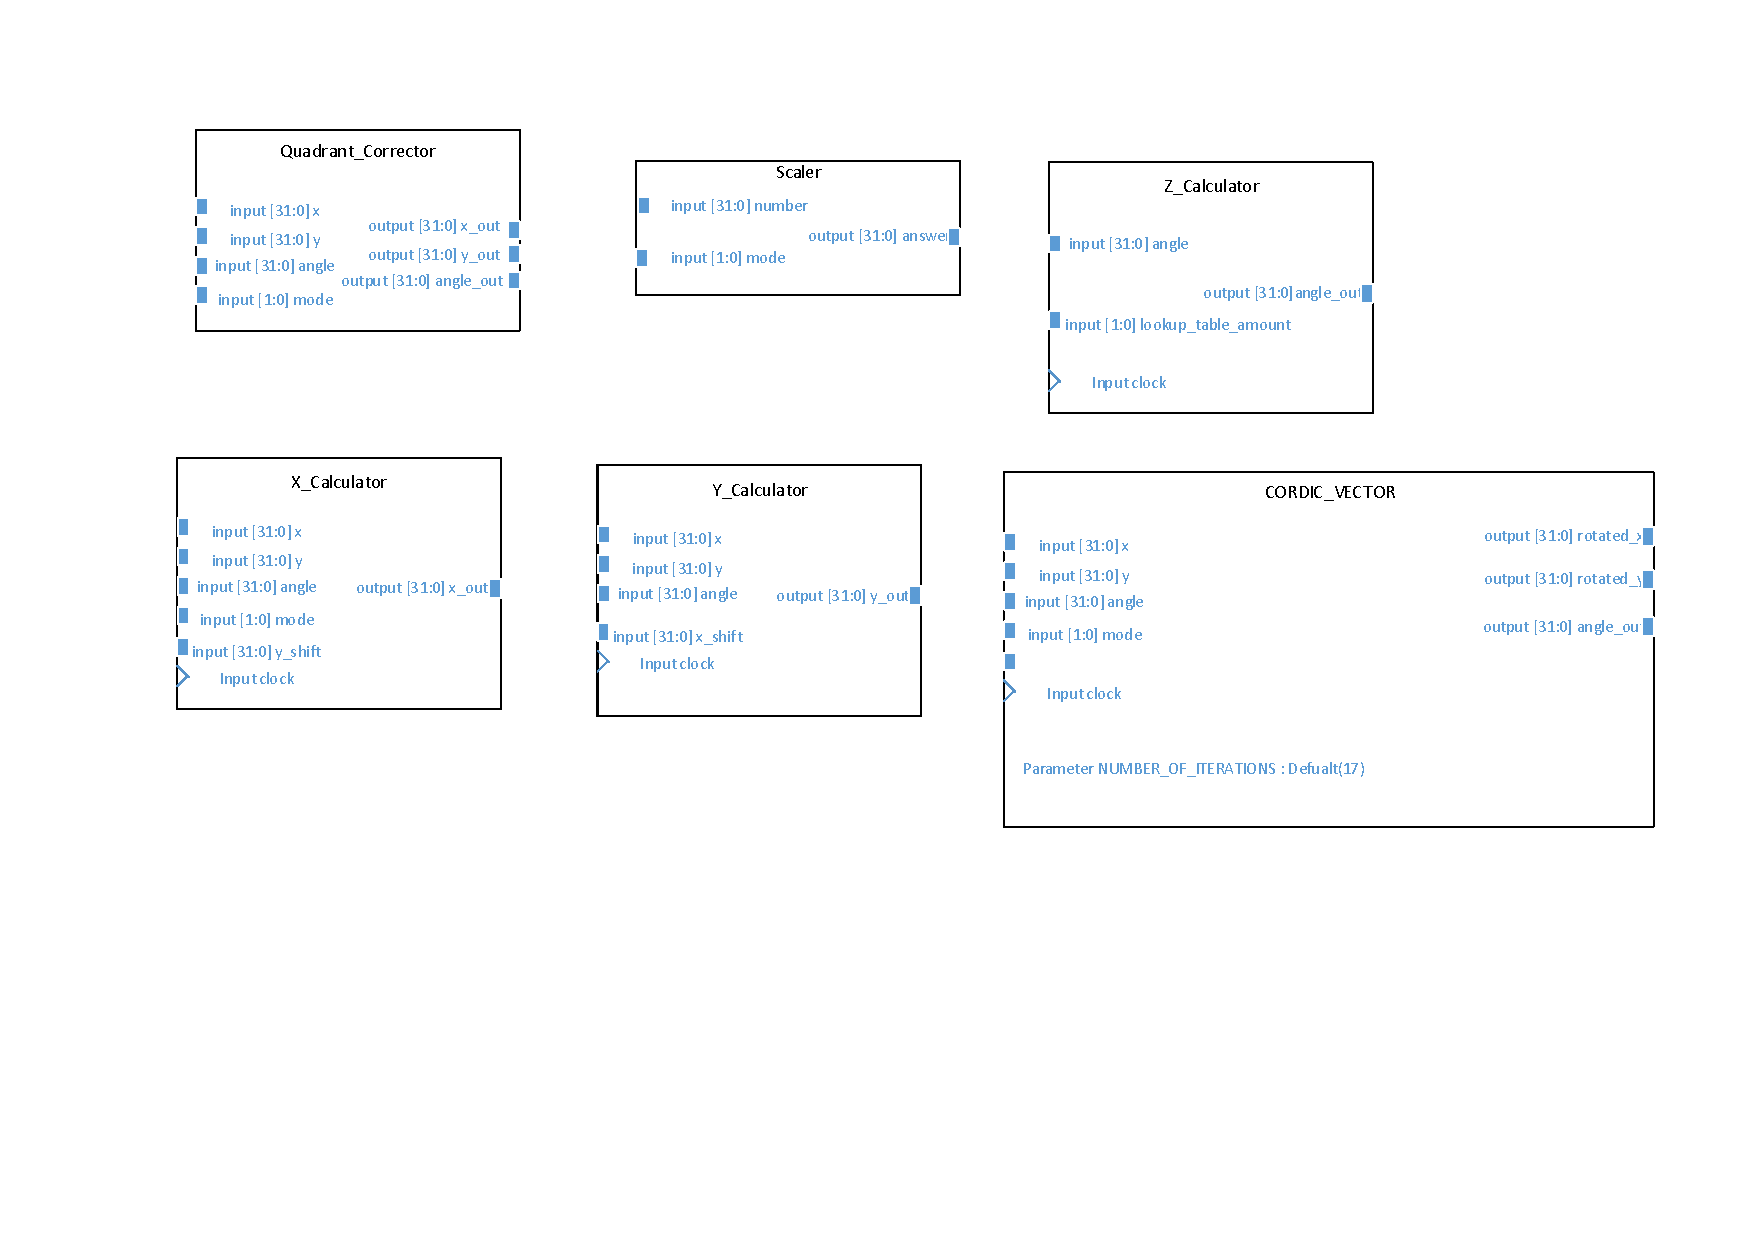
\includepdf[pages=1,angle=90, ]{CORDICVECTOR.pdf}


\end{landscape}


\newpage

\begin{landscape}

\thispagestyle{empty}
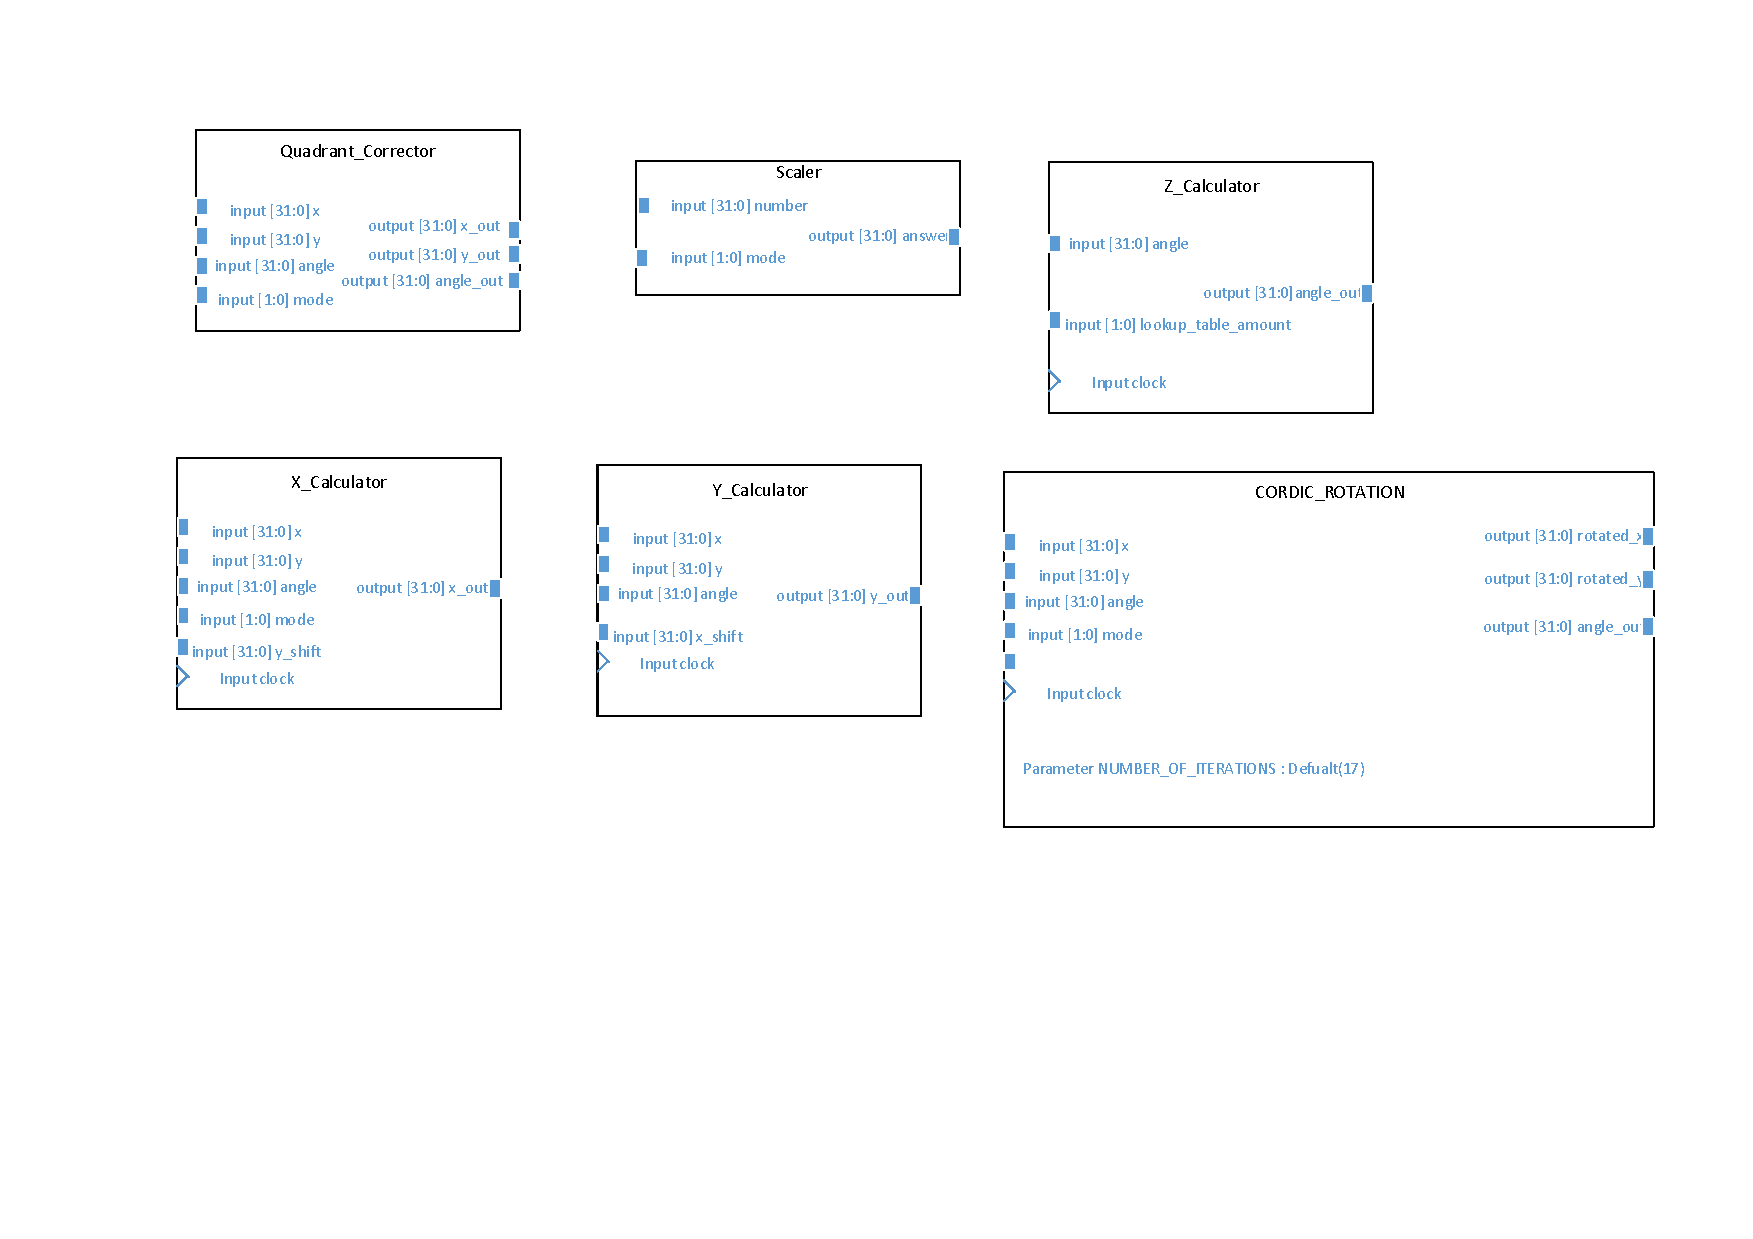
\includepdf[pages=1,angle=90, ]{CORDICROTATION.pdf}

\end{landscape}
\newpage



\begin{landscape}
\thispagestyle{empty}

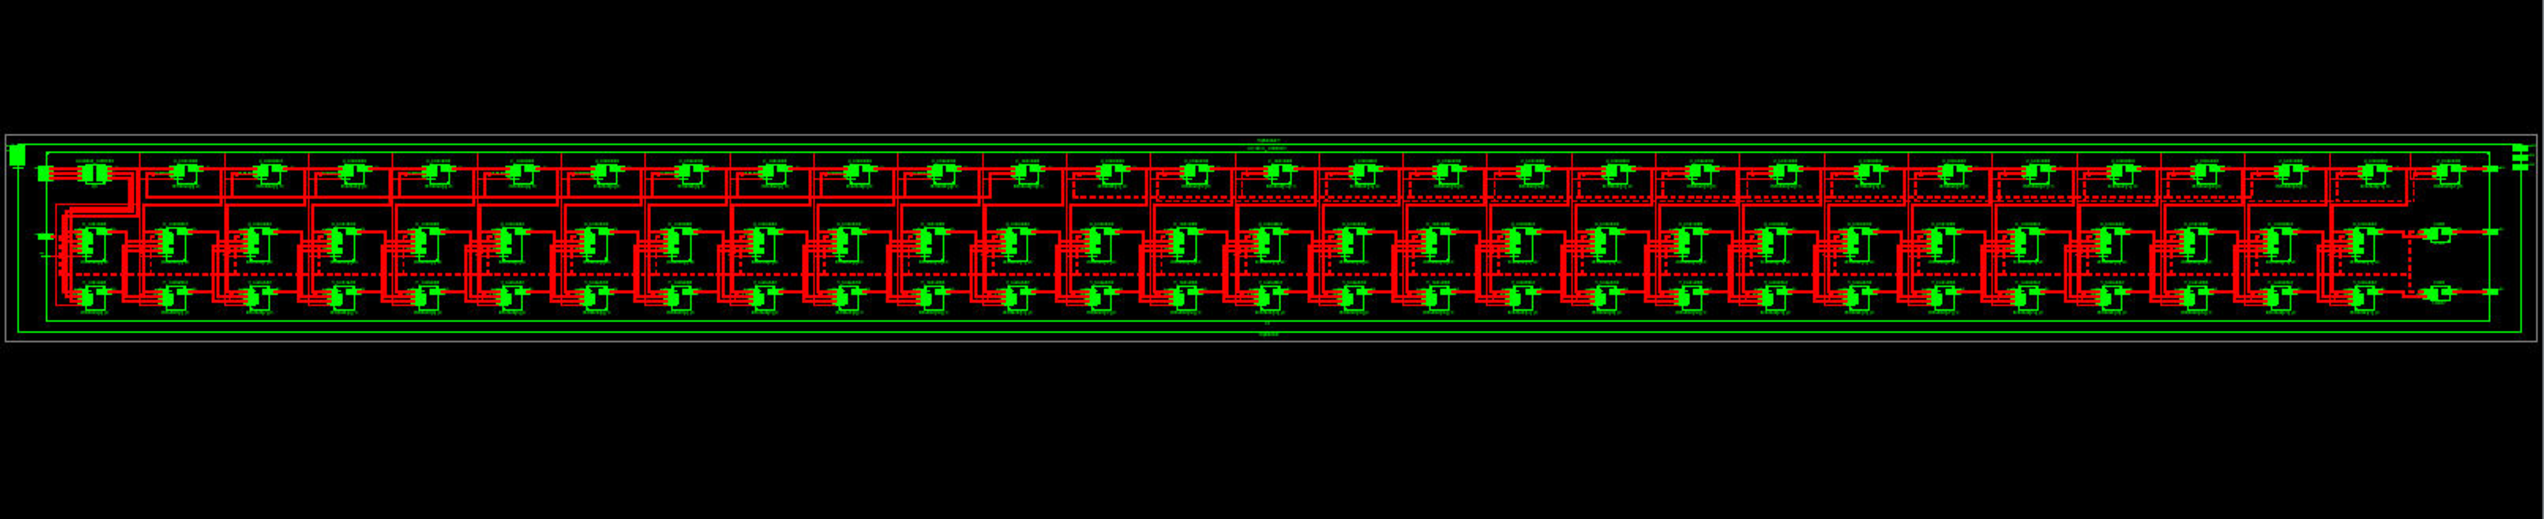
\includepdf[pages=1,angle=90, ]{BigPicture_Rotation.pdf}
\end{landscape}

\begin{landscape}
\thispagestyle{empty}

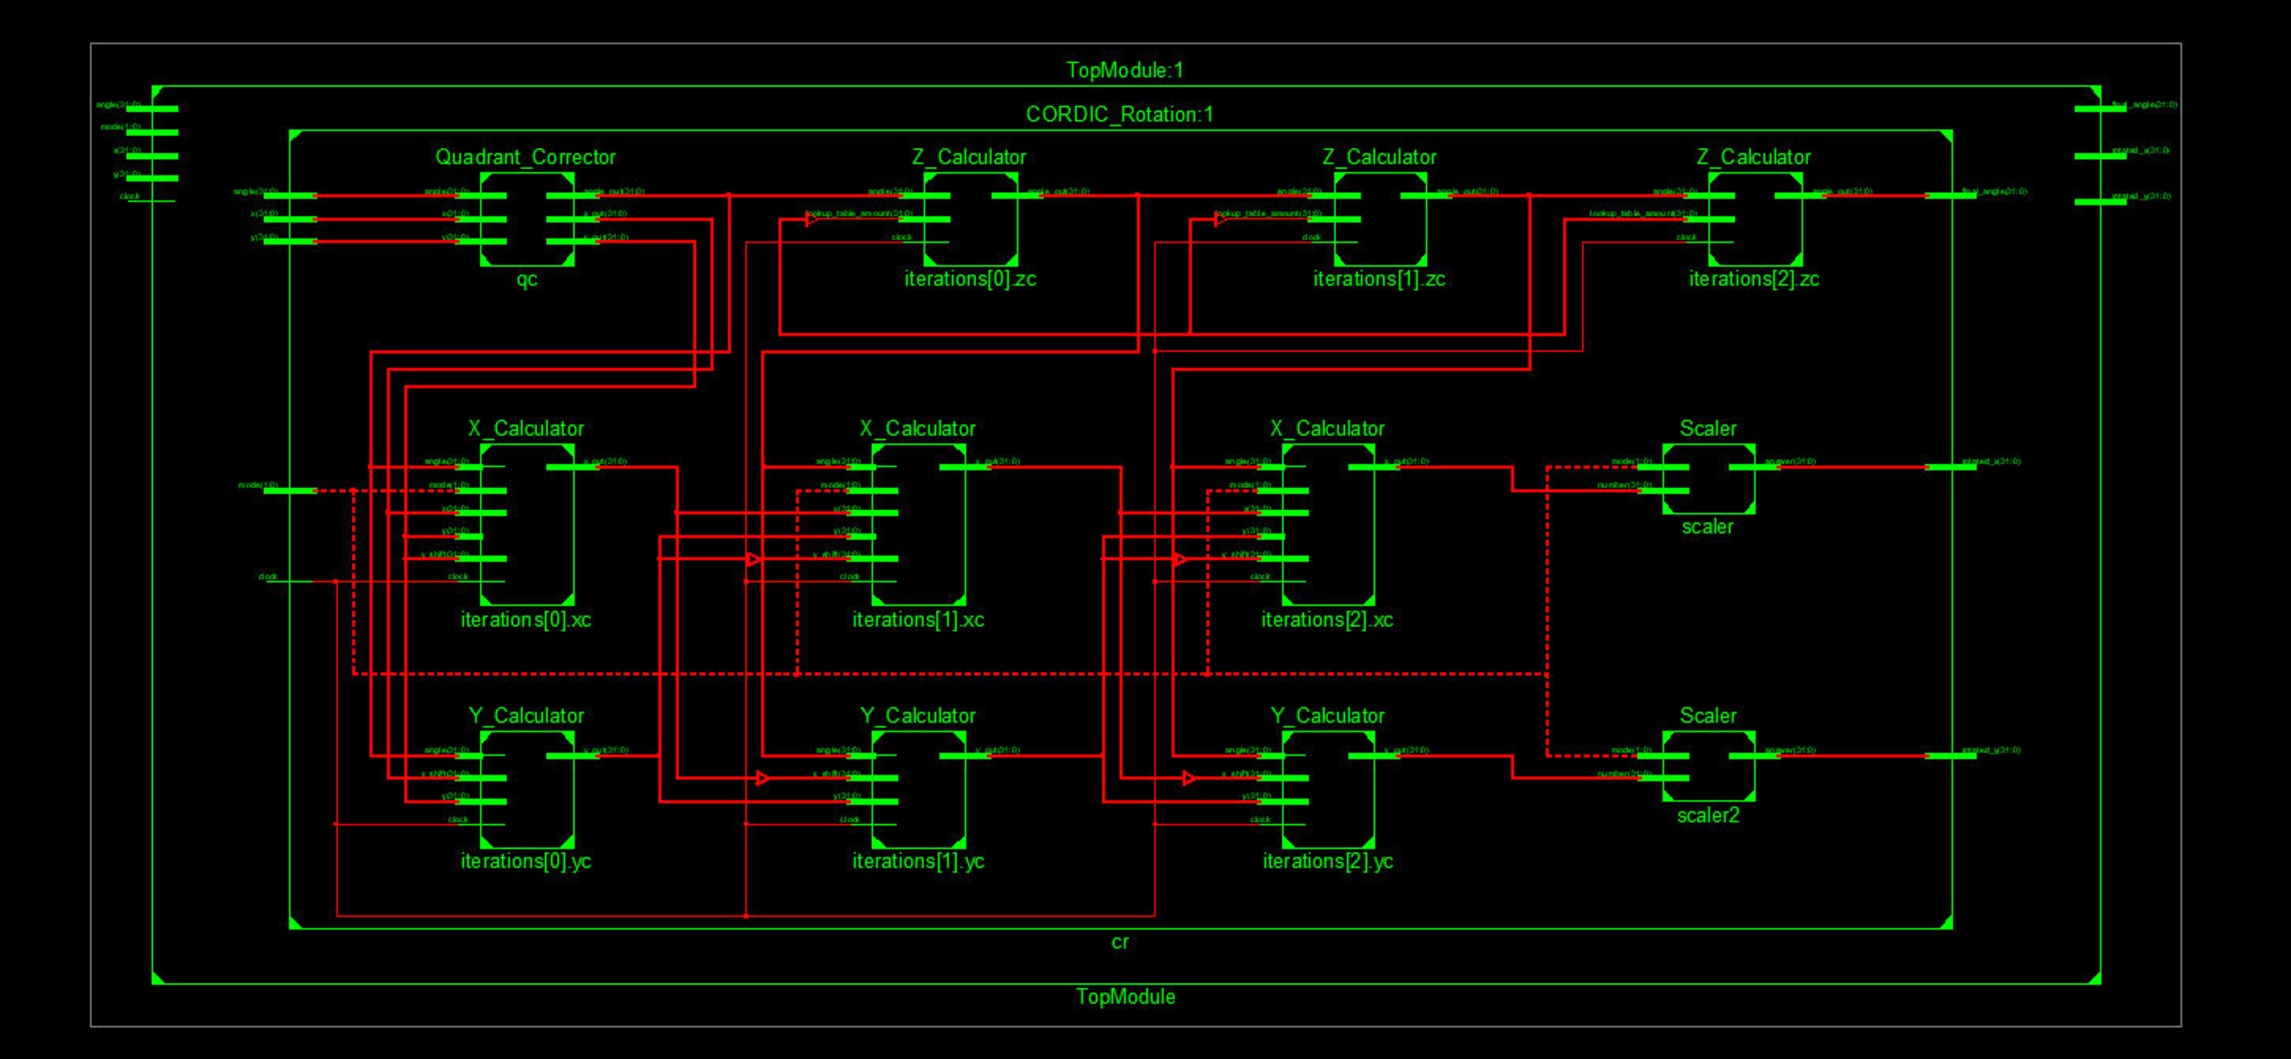
\includepdf[pages=1,angle=90, ]{CORDIC_SMALL.pdf}
\end{landscape}

\begin{landscape}
\thispagestyle{empty}

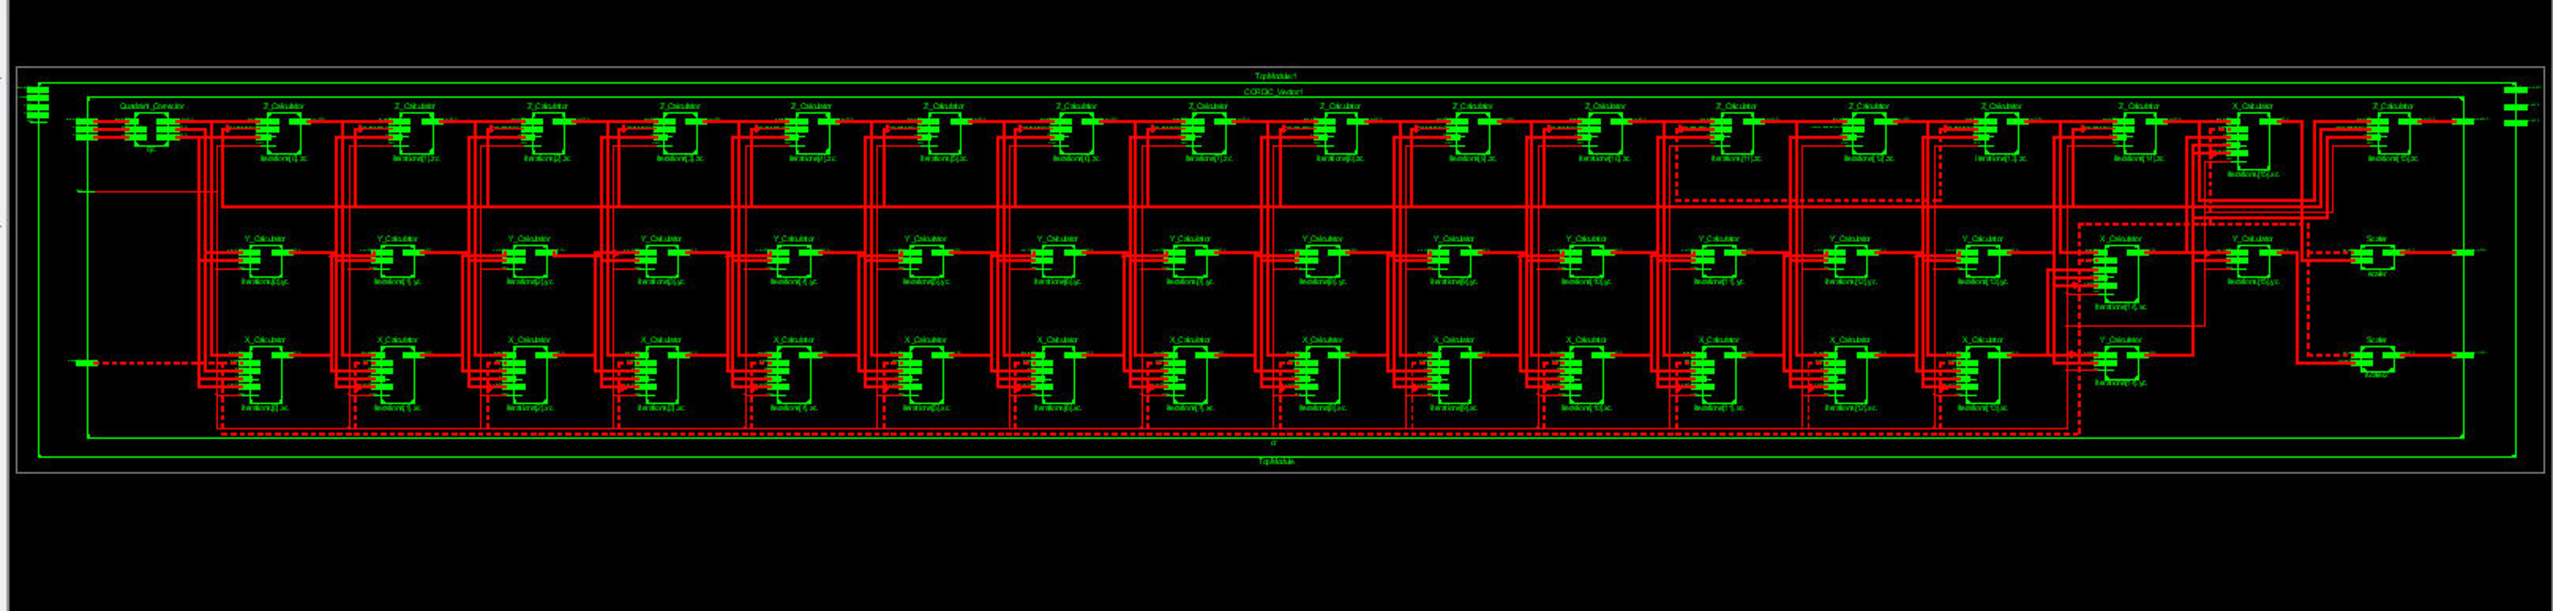
\includepdf[pages=1,angle=90, ]{BigPicture_Vector.pdf}
\end{landscape}

\begin{landscape}
\thispagestyle{empty}

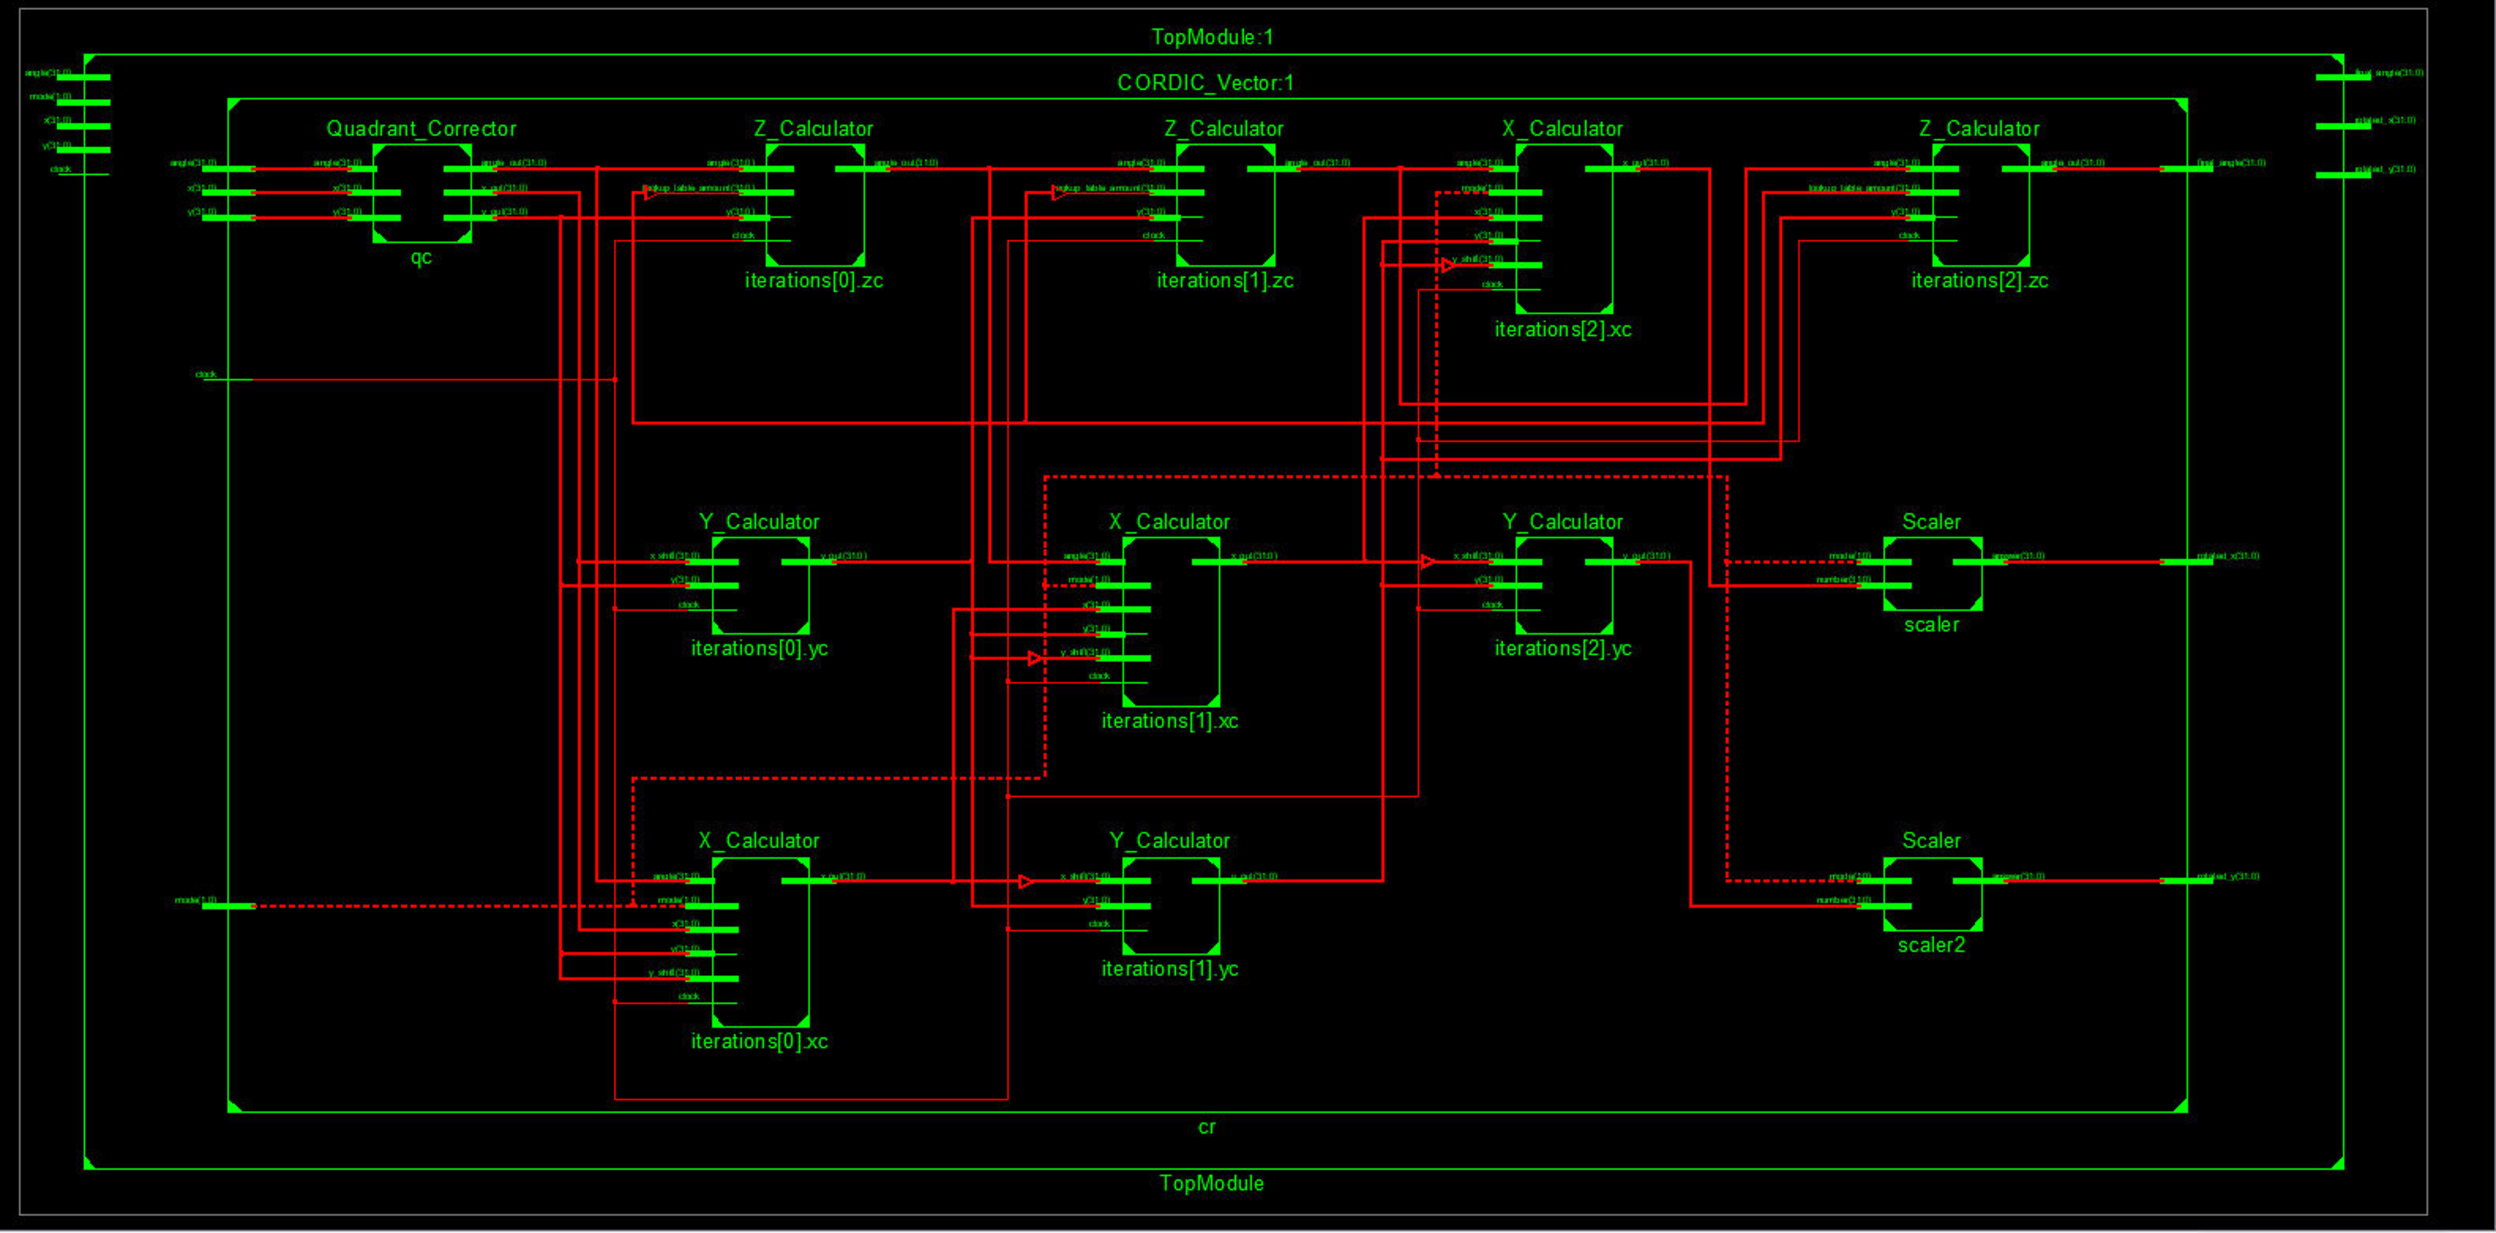
\includepdf[pages=1,angle=90, ]{CORDIC_VECTOR_SMALL.pdf}
\end{landscape}


\subsection{شرح وظایف ماژول‌ها}

در فایل‌های قرار داده شده، دو پوشه جدا داریم. یکی Rotation و دیگری Vectoring که هر کدام مختص به پروژه مربوط به خود هستند. البته ساختار بسیاری از ماژول‌های آنان، مشابه است اما از آن جایی که دو پروژه مجزا بودند، ما هم آنان را به صورت دو پوشه و پروژه مجزا قرار داده‌ایم. اما پیش از توضیح در مورد خود ماژول‌ها، باید در مورد نحوه انکود کردن اعداد به صورت باینری توضیح داده بشود.

برای انکود کردن زاویه‌ها، آن‌ها را بر $360$ تقسیم کرده و سپس در $2^{31}$ ضرب می‌کنیم و عدد حاصل را به صورت $32$ بیتی نمایش می‌دهیم. یعنی با فرمول زیر:
$$\frac{\text{Angle}}{360} \times 2^{31} \rightarrow 32 ~~\text{\lr{bit binary number}}$$
 مثلاً زوایای $45$ درجه، $135$ درجه، $225$ درجه و $315$ درجه، به شکل زیر می‌شوند:

\begin{latin}
\begin{verbatim}

 45 deg: 32'b00010000000000000000000000000000
135 deg: 32'b00110000000000000000000000000000
225 deg: 32'b01010000000000000000000000000000
315 deg: 32'b01110000000000000000000000000000

\end{verbatim}
\end{latin} 

برای تبدیل برعکس آن هم عدد باینری را به صورت یک Integer در نظر می‌گیریم و عدد به دست آمده را بر $2^{31}$ تقسیم کرده و ضربدر $360$ می‌کنیم.


دلیل این که ضرب را در $2^{31}$ انجام دادیم و نه $2^{32}$، این است که در حالت Linear نیاز به  تبدیل عدد $2^{0}$ به مقیاس انکود شده در بالا به دست می آمده است و اگر در $2^{32}$ ضرب انجام می‌شد، با مشکل Overflow رو به رو می‌شدیم.

اعداد $x$ و $y$ هم به شکل Fixed-Point با $12$ رقم صحیح و $20$ رقم اعشاری انکود شده‌اند. در نتیجه برای تبدیل یک عدد به حالت نمایش داده شده $32$ بیتی باید از فرمول زیر استفاده کرد:

$$\text{Number} \times 2^{20} \rightarrow 32 ~~\text{\lr{bit binary number}}$$

و برای تبدیل برعکس هم باید عدد باینری $32$ بیتی گرفته شده را به صورت Integer در نظر گرفته و بر $2^{20}$ تقسیم کرد.

مثلاً عدد $120$، $2$ و $170.5$ در این انکودینگ به شکل زیر نمایش داده می‌شود.
 
 
 \begin{latin}
\begin{verbatim}

  120: 32'b000001111000\_00000000000000000000
    2: 32'b000000000010\_00000000000000000000
170.5: 32'b000010101010\_10000000000000000000
\end{verbatim}
\end{latin} 

 
\subsubsection{Vectoring}

قبل از اشاره به ماژول‌های اصلی پروژه، می‌بایست به فایل ثوابت یا \lr{CONSTANTS.v} اشاره کنیم. در این فایل از طریق \lr{`define} سه ثابت به صورت زیر تعریف شده است:
\begin{latin}
\begin{verbatim}
`define CIRCULAR 2'b01
`define LINEAR 2'b00
`define HYPERBOLIC 2'b11
\end{verbatim}
\end{latin}

این فایل از طریق \lr{`include} در سایر ماژول‌ها قرار گرفته است.

ماژول‌ها را در ادامه به ترتیب Bottom-Up شرح می‌دهیم.

اولین ماژول \lr{Quadrant\_Corrector} است که در فایل هم نام خودش قرار دارد. 

 ورودی‌های آن موارد زیر هستند:

\begin{latin}
\begin{verbatim}
input [31:0] x,
input [31:0] y,
input[31:0] angle,
\end{verbatim}
\end{latin}

و خروجی‌های آن:

\begin{latin}
\begin{verbatim}
output reg [31:0] x_out,
output reg [31:0] y_out,
output reg [31:0] angle_out
\end{verbatim}
\end{latin}

وظیفه این ماژول این است که اگر $x$ و $y$ ورودی در ناحیه اول یا چهارم قرار نداشتند، از طریق تبدیل‌هایی که در بخش ریاضی نوشتیم، آن‌ها را به ناحیه اول یا چهارم منتقل کرده و برای حالتی که در ناحیه دوم باشند، زاویه اولیه خروجی را $90$ درجه و در حالتی که در ناحیه سوم باشند، زاویه اولیه خروجی را $270$ درجه (معادل $-90$ درجه) قرار بدهد.

\hrulefill

ماژول بعدی \lr{Scaler} است که در فایل هم نام خودش قرار دارد.

 
 ورودی‌های آن موارد زیر هستند:

\begin{latin}
\begin{verbatim}
input [31:0] number,
input [1:0] mode
\end{verbatim}
\end{latin}

و خروجی آن:

\begin{latin}
\begin{verbatim}
output [31:0] answer
\end{verbatim}
\end{latin}

است. ورودی mode بیانگر این است که وضعیت برنامه در حالت CIRCULAR یا HYPERBOLIC یا LINEAR قرار دارد و بر اساس ثابت‌های \lr{CONSTANTS.v} مشخص می‌شود. وظیفه کلی این ماژول این است که عدد داده شده را متناسب با حالت داده شده در ضریب $K$ مناسب ضرب کند. برای حالت CIRCULAR این $K$ برابر $0.6073$ برای HYPERBOLIC برابر $1.2075$ و در حالت LINEAR برابر $1$ است. برای این که در ضرب کردن، از ماژول ضرب کننده استفاده نکنیم، برای ضرب در این اعداد از ترکیب شیفت و جمع استفاده می‌کنیم. به عنوان مثال
$$0.6073 \approx 2^{-1} + 2^{-4} + 2^{-5} + 2^{-7} + 2^{-7} + 2^{-10} + 2^{-11} + 2^{-12} + 2^{-13}$$
است در نتیجه، این جمع را به این شکل انجام می‌دهیم:

\begin{latin}
\begin{verbatim}
(number >>> 1) +(number >>>4) + (number>>>5)
+ (number>>>7) + (number>>>8) + (number>>>10) +
 (number>>>11) + (number>>>12) + (number>>>13);
\end{verbatim}
\end{latin}

در مورد $1.2075$ هم روش مشابهی اعمال می‌کنیم، با این تفاوت که وجود $1$ در عدد $1.2075$ یعنی یکی از بخش‌های جمع شونده، خود عدد اصلی بدون هیچ نوع شیفت اضافی است.

\hrulefill

ماژول بعدی \lr{X\_Calculator} است که در فایل هم نام خودش قرار دارد.

 
 ورودی‌های آن موارد زیر هستند:

\begin{latin}
\begin{verbatim}
input[31:0] x,
input[31:0] y,
input [31:0] angle,
input [1:0] mode,
input [31:0] y_shift,
input clock
\end{verbatim}
\end{latin}

و خروجی آن:

\begin{latin}
\begin{verbatim}
output [31:0] x_out
\end{verbatim}
\end{latin}

سه ورودی اول که مشخص هستند. ورودی چهارم مربوط به همین است که در حالت CIRCULAR هستیم یا HYPERBOLIC یا LINEAR. ورودی پنجم که \lr{y\_shift} است، در اصل همان مقدار $y_i \times 2^{-i}$ در فرمول‌هاست که از ماژول اصلی به عنوان ورودی وارد این ماژول می‌شود. در نهایت هم clock را داریم که برای اجرای مرحله به مرحله سیستم به صورت \lr{Pipeline}، وجود کلاک که باعث ذخیره شدن و باقی ماندن مقادیر در رجیسترها بشود، ضروری است.

درون این ماژول بر اساس ورودی‌های داده شده، محاسبات طبق فرمول‌های بخش ریاضی و بر اساس علامت $y$ انجام شده و مقدار جدید $x$ تحت نام \lr{x\_out} خروجی داده می‌شود.

\hrulefill
 

ماژول بعدی \lr{Y\_Calculator} است که در فایل هم نام خودش قرار دارد.

 
 ورودی‌های آن موارد زیر هستند:

\begin{latin}
\begin{verbatim}
input[31:0] x,
input[31:0] y,
input [31:0] angle,
input [31:0] x_shift,
input clock
\end{verbatim}
\end{latin}

و خروجی آن:

\begin{latin}
\begin{verbatim}
output [31:0] y_out
\end{verbatim}
\end{latin}

این ماژول از نظر ورودی‌ها کاملاً مشابه \lr{X\_Calculator} است، با این تفاوت که از آن جایی که نیازی به جز این که در این جا نیازی به دانستن mode نداریم و به عنوان ورودی داده نشده است. هدف این ماژول هم انجام محاسبات مربوط به $y$ است.

\hrulefill


ماژول بعدی \lr{Z\_Calculator} است که در فایل هم نام خودش قرار دارد.

 
 ورودی‌های آن موارد زیر هستند:

\begin{latin}
\begin{verbatim}
input [31:0] angle,
input [31:0] y,
input [31:0] lookup_table_amount,
input clock,
\end{verbatim}
\end{latin}

و خروجی آن:

\begin{latin}
\begin{verbatim}
 output wire [31:0] angle_out
\end{verbatim}
\end{latin}

این ماژول هم از نظر عملکردی، مشابه دو ماژول قبلی است. تنها نکته این جاست که یک مقدار تحت نام \lr{lookup\_table\_amount} به آن ورودی داده می‌شود که در اصل، مقداری برابر با $2^{-i}$ یا $\arctan (2^{-1})$ یا
$\arctanh (2^{-1})$
است که از طریق یک تابع در ماژول اصلی تولید شده و به بسته به مود کلی سیستم، به عنوان ورودی به این ماژول که محاسبه کننده $Z$ یا همان $angle$ و زاویه بعدی است، داده می‌شود.

\hrulefill

فایل ماژول اصلی این پروژه، \lr{CORDIC\_Vector} نام دارد. ورودی‌های آن موارد زیر هستند:

\begin{latin}
\begin{verbatim}
input signed [31:0] x,
input signed [31:0] y,
input signed [31:0] angle,
input [1:0] mode
\end{verbatim}
\end{latin}

و خروجی‌های آن:

\begin{latin}
\begin{verbatim}
 output wire signed [31:0] rotated_x,
 output wire signed [31:0] rotated_y,
 output wire signed [31:0] final_angle
\end{verbatim}
\end{latin}

هستند. دلیل این که 32 بیتی در نظر گرفتیم، این بود که در حالت 16 بیتی، برای بسیاری از ورودی‌ها خروجی برنامه دقت کافی را نداشت.

پارامتر برنامه هم:

\begin{latin}
\begin{verbatim}
parameter NUMBER_OF_ITERATIONS = 17;
\end{verbatim}
\end{latin}

است. مقدار پیش فرض 17 از این رو قرار گرفته است که بهترین نتیجه‌ای که در تست‌های مختلف دریافت کردیم، برای ورودی و خروجی 32 بیتی، در حالت Vectoring مقدار 17، نتیجه مناسبی ارائه می‌داد و مقادیر بیش‌تر بعضاً منجر به ایجاد Overflow در محاسبات شده و مقادیر کمتر هم دقت را کاهش می‌دادند.


ابتدا به تعداد Iteration های برنامه، یک آرایه از Vector های 32 بیتی Wire برای ایجاد ارتباطات میان خروجی $x,y,angle$ مراحل مختلف ایجاد کرده‌ایم که \lr{x\_prime}، \lr{y\_prime} و \lr{rotated\_angles} نام دارند.

در ابتدا، یک Instance از ماژول \lr{Quadrant\_Corrector} ساخته شده که وضعیت زاویه و ورودی‌های اصلی برنامه را مشخص کند و مقادیر خروجی آن، به مقادیر اندیس صفر  \lr{x\_prime}، \lr{y\_prime} و \lr{rotated\_angles} وصل می‌شوند.

سپس از طریق Generate به تعداد Iteration هایی که از طریق پارامتر تعریف شده است، instance از ماژول \lr{Y\_Calculator}، \lr{X\_Calculator} و \lr{Z\_Calculator} ساخته‌ایم. یکسری متغیر temp هم وجود دارند که مقادیر مربوط به $\arctan$ یا $\arctanh$ و همچنین شیفت داده شده $X$ و $Y$ به اندازه $i$ را که اندیس همان مرحله باشد، به عنوان وردی به این ماژول‌ها متصل کنند.

بعد از بخش Generate، دو Instance از \lr{Scaler} ساخته شده که خروجی‌های مرحله آخر ماژول‌ها که یعنی اندیس
$NUMBER\_OF\_ITERATIONS - 1$
ام
 \lr{x\_prime}،
  \lr{y\_prime} به آن‌ها وصل شده تا متناسب با mode با ضریب $K$ مشخص Scale بشوند.

در نهایت این خروجی‌ها به عنوان خروجی اصلی برنامه داده شده‌اند.

در انتهای این کد، یک تابع به نام Lookup وجود دارد که Index و mode را ورودی گرفته و بر اساس آن، مقدار متناسب را از بین جدول $\arctan$ یا $\arctanh$ یا $2^{-i}$ خروجی می‌دهد. دلیل این که از تابع استفاده کردیم، این است که در اصل مقادیر این تابع، به عنوان یکسری ثابت که از طریق Mux انتخاب می‌شوند، در حین Instantiate شدن ماژول‌های درون Generate به آن‌ها داده می‌شوند و نیازی نیست که از یک ROM جداگانه استفاده کنیم. زیرا در صورت استفاده از ROM باید امکان خوانده شدن همزمان حدود 32 مقدار مختلف را در بدترین حالت برای آن فراهم می‌کردیم تا همه مراحل سیستم بتوانند به صورت Pipeline و مستقل از هم کار بکنند که هزینه اجرایی بالایی داشت و از این رو آن را به صورت تابع پیاده‌سازی کردیم.


\hrulefill

\newpage
در نهایت یک \lr{Top Module} با نام \lr{TopModule} داریم که ورودی‌های آن به صورت زیر است:

\begin{latin}

\begin{verbatim}
input signed [31:0] x,
input signed [31:0] y,
input signed [31:0] angle,
input [1:0] mode,
   
\end{verbatim}

\end{latin}


و خروجی‌های آن:


\begin{latin}

\begin{verbatim}
output wire signed [31:0] rotated_x,
output wire signed [31:0] rotated_y,
output wire signed [31:0] final_angle
   
\end{verbatim}

\end{latin}

در این ماژول فقط یک Instance از CORDIC\_Vector با اندازه پارامتر مشخص ساخته شده که در سنتز و تست بنچ مورد استفاده قرار بگیرد.


\newpage
\subsubsection{ROTATION}
بخش زیادی از ماژول‌های استفاده شده در این بخش، مشابه بخش قبل است اما برای کامل بودن گزارش، توضیحات آن‌ها مجدداً مانند بخش قبل آورده شده است.




قبل از اشاره به ماژول‌های اصلی پروژه، می‌بایست به فایل ثوابت یا \lr{CONSTANTS.v} اشاره کنیم. در این فایل از طریق \lr{`define} سه ثابت به صورت زیر تعریف شده است:
\begin{latin}
\begin{verbatim}
`define CIRCULAR 2'b01
`define LINEAR 2'b00
`define HYPERBOLIC 2'b11
\end{verbatim}
\end{latin}

این فایل از طریق \lr{`include} در سایر ماژول‌ها قرار گرفته است.

ماژول‌ها را در ادامه به ترتیب Bottom-Up شرح می‌دهیم.

اولین ماژول \lr{Quadrant\_Corrector} است که در فایل هم نام خودش قرار دارد. 

 ورودی‌های آن موارد زیر هستند:

\begin{latin}
\begin{verbatim}
input [31:0] x,
input [31:0] y,
input[31:0] angle,
\end{verbatim}
\end{latin}

و خروجی‌های آن:

\begin{latin}
\begin{verbatim}
output reg [31:0] x_out,
output reg [31:0] y_out,
output reg [31:0] angle_out
\end{verbatim}
\end{latin}

وظیفه این ماژول این است که اگر زاویه داده شده در بازه
 $\frac{-\pi}{2} < angle < \frac{\pi}{2}$
 یا به بیان دیگر،
 $270 < angle \leq 360$
 یا
 $0 \leq angle <90$
 قرار نداشت،
یعنی تبدیل متناسب با ناحیه اول و چهارم قرار نداشت، از طریق تبدیل‌هایی که در بخش ریاضی نوشتیم، آن‌ها را به ناحیه اول یا چهارم منتقل کرده و برای حالتی که در ناحیه دوم باشند، زاویه اولیه خروجی را $90$ درجه کم کرده و در حالتی که در ناحیه سوم باشند، زاویه اولیه خروجی را $90$ درجه افزایش بدهد (به بیان دیگر $270$ درجه کم کند) تا در ناحیه چهارم قرار بگیرد و متناسب با آن تغییرات را روی $x$ و $y$ هم اعمال کند.


\hrulefill

ماژول بعدی \lr{Scaler} است که در فایل هم نام خودش قرار دارد.

 
 ورودی‌های آن موارد زیر هستند:

\begin{latin}
\begin{verbatim}
input [31:0] number,
input [1:0] mode
\end{verbatim}
\end{latin}

و خروجی آن:

\begin{latin}
\begin{verbatim}
output [31:0] answer
\end{verbatim}
\end{latin}

است. ورودی mode بیانگر این است که وضعیت برنامه در حالت CIRCULAR یا HYPERBOLIC یا LINEAR قرار دارد و بر اساس ثابت‌های \lr{CONSTANTS.v} مشخص می‌شود. وظیفه کلی این ماژول این است که عدد داده شده را متناسب با حالت داده شده در ضریب $K$ مناسب ضرب کند. برای حالت CIRCULAR این $K$ برابر $0.6073$ برای HYPERBOLIC برابر $1.2075$ و در حالت LINEAR برابر $1$ است. برای این که در ضرب کردن، از ماژول ضرب کننده استفاده نکنیم، برای ضرب در این اعداد از ترکیب شیفت و جمع استفاده می‌کنیم. به عنوان مثال
$$0.6073 \approx 2^{-1} + 2^{-4} + 2^{-5} + 2^{-7} + 2^{-7} + 2^{-10} + 2^{-11} + 2^{-12} + 2^{-13}$$
است در نتیجه، این جمع را به این شکل انجام می‌دهیم:

\begin{latin}
\begin{verbatim}
(number >>> 1) +(number >>>4) + (number>>>5)
+ (number>>>7) + (number>>>8) + (number>>>10) +
 (number>>>11) + (number>>>12) + (number>>>13);
\end{verbatim}
\end{latin}

در مورد $1.2075$ هم روش مشابهی اعمال می‌کنیم، با این تفاوت که وجود $1$ در عدد $1.2075$ یعنی یکی از بخش‌های جمع شونده، خود عدد اصلی بدون هیچ نوع شیفت اضافی است.

\hrulefill

ماژول بعدی \lr{X\_Calculator} است که در فایل هم نام خودش قرار دارد.

 
 ورودی‌های آن موارد زیر هستند:

\begin{latin}
\begin{verbatim}
input[31:0] x,
input[31:0] y,
input [31:0] angle,
input [1:0] mode,
input [31:0] y_shift,
input clock
\end{verbatim}
\end{latin}

و خروجی آن:

\begin{latin}
\begin{verbatim}
output [31:0] x_out
\end{verbatim}
\end{latin}

سه ورودی اول که مشخص هستند. ورودی چهارم مربوط به همین است که در حالت CIRCULAR هستیم یا HYPERBOLIC یا LINEAR. ورودی پنجم که \lr{y\_shift} است، در اصل همان مقدار $y_i \times 2^{-i}$ در فرمول‌هاست که از ماژول اصلی به عنوان ورودی وارد این ماژول می‌شود. در نهایت هم clock را داریم که برای اجرای مرحله به مرحله سیستم به صورت \lr{Pipeline}، وجود کلاک که باعث ذخیره شدن و باقی ماندن مقادیر در رجیسترها بشود، ضروری است.

درون این ماژول بر اساس ورودی‌های داده شده، محاسبات طبق فرمول‌های بخش ریاضی بر اساس علامت $angle$ که با توجه به فرمت خاصی که برای انکود کردن انتخاب کردیم، در بیت $31$ ام آن (اندیس $30$) قرار دارد، انجام شده و مقدار جدید $x$ تحت نام \lr{x\_out} خروجی داده می‌شود.

\hrulefill
 

ماژول بعدی \lr{Y\_Calculator} است که در فایل هم نام خودش قرار دارد.

 
 ورودی‌های آن موارد زیر هستند:

\begin{latin}
\begin{verbatim}
input[31:0] x,
input[31:0] y,
input [31:0] angle,
input [31:0] x_shift,
input clock
\end{verbatim}
\end{latin}

و خروجی آن:

\begin{latin}
\begin{verbatim}
output [31:0] y_out
\end{verbatim}
\end{latin}

این ماژول از نظر ورودی‌ها کاملاً مشابه \lr{X\_Calculator} است، با این تفاوت که از آن جایی که نیازی به جز این که در این جا نیازی به دانستن mode نداریم و به عنوان ورودی داده نشده است. هدف این ماژول هم انجام محاسبات مربوط به $y$ است.

\hrulefill


ماژول بعدی \lr{Z\_Calculator} است که در فایل هم نام خودش قرار دارد.

 
 ورودی‌های آن موارد زیر هستند:

\begin{latin}
\begin{verbatim}
input [31:0] angle,
input [31:0] y,
input [31:0] lookup_table_amount,
input clock,
\end{verbatim}
\end{latin}

و خروجی آن:

\begin{latin}
\begin{verbatim}
 output wire [31:0] angle_out
\end{verbatim}
\end{latin}

این ماژول هم از نظر عملکردی، مشابه دو ماژول قبلی است. تنها نکته این جاست که یک مقدار تحت نام \lr{lookup\_table\_amount} به آن ورودی داده می‌شود که در اصل، مقداری برابر با $2^{-i}$ یا $\arctan (2^{-1})$ یا
$\arctanh (2^{-1})$
است که از طریق یک تابع در ماژول اصلی تولید شده و به بسته به مود کلی سیستم، به عنوان ورودی به این ماژول که محاسبه کننده $Z$ یا همان $angle$ و زاویه بعدی است، داده می‌شود.

\hrulefill

فایل ماژول اصلی این پروژه، \lr{CORDIC\_Rotation} نام دارد. ورودی‌های آن موارد زیر هستند:

\begin{latin}
\begin{verbatim}
input signed [31:0] x,
input signed [31:0] y,
input signed [31:0] angle,
input [1:0] mode
\end{verbatim}
\end{latin}

و خروجی‌های آن:

\begin{latin}
\begin{verbatim}
 output wire signed [31:0] rotated_x,
 output wire signed [31:0] rotated_y,
 output wire signed [31:0] final_angle
\end{verbatim}
\end{latin}

هستند. دلیل این که 32 بیتی در نظر گرفتیم، این بود که در حالت 16 بیتی، برای بسیاری از ورودی‌ها خروجی برنامه دقت کافی را نداشت.

پارامتر برنامه هم:

\begin{latin}
\begin{verbatim}
parameter NUMBER_OF_ITERATIONS = 29;
\end{verbatim}
\end{latin}


ابتدا به تعداد Iteration های برنامه، یک آرایه از Vector های 32 بیتی Wire برای ایجاد ارتباطات میان خروجی $x,y,angle$ مراحل مختلف ایجاد کرده‌ایم که \lr{x\_prime}، \lr{y\_prime} و \lr{rotated\_angles} نام دارند.

در ابتدا، یک Instance از ماژول \lr{Quadrant\_Corrector} ساخته شده که وضعیت زاویه و ورودی‌های اصلی برنامه را مشخص کند و مقادیر خروجی آن، به مقادیر اندیس صفر  \lr{x\_prime}، \lr{y\_prime} و \lr{rotated\_angles} وصل می‌شوند.

سپس از طریق Generate به تعداد Iteration هایی که از طریق پارامتر تعریف شده است، instance از ماژول \lr{Y\_Calculator}، \lr{X\_Calculator} و \lr{Z\_Calculator} ساخته‌ایم. یکسری متغیر temp هم وجود دارند که مقادیر مربوط به $\arctan$ یا $\arctanh$ و همچنین شیفت داده شده $X$ و $Y$ به اندازه $i$ را که اندیس همان مرحله باشد، به عنوان وردی به این ماژول‌ها متصل کنند.

بعد از بخش Generate، دو Instance از \lr{Scaler} ساخته شده که خروجی‌های مرحله آخر ماژول‌ها که یعنی اندیس
$NUMBER\_OF\_ITERATIONS - 1$
ام
 \lr{x\_prime}،
  \lr{y\_prime} به آن‌ها وصل شده تا متناسب با mode با ضریب $K$ مشخص Scale بشوند.

در نهایت این خروجی‌ها به عنوان خروجی اصلی برنامه داده شده‌اند.

در انتهای این کد، یک تابع به نام Lookup وجود دارد که Index و mode را ورودی گرفته و بر اساس آن، مقدار متناسب را از بین جدول $\arctan$ یا $\arctanh$ یا $2^{-i}$ خروجی می‌دهد. دلیل این که از تابع استفاده کردیم، این است که در اصل مقادیر این تابع، به عنوان یکسری ثابت که از طریق Mux انتخاب می‌شوند، در حین Instantiate شدن ماژول‌های درون Generate به آن‌ها داده می‌شوند و نیازی نیست که از یک ROM جداگانه استفاده کنیم. زیرا در صورت استفاده از ROM باید امکان خوانده شدن همزمان حدود 32 مقدار مختلف را در بدترین حالت برای آن فراهم می‌کردیم تا همه مراحل سیستم بتوانند به صورت Pipeline و مستقل از هم کار بکنند که هزینه اجرایی بالایی داشت و از این رو آن را به صورت تابع پیاده‌سازی کردیم.


\hrulefill

در نهایت یک \lr{Top Module} با نام \lr{TopModule} داریم که ورودی‌های آن به صورت زیر است:

\begin{latin}

\begin{verbatim}
input signed [31:0] x,
input signed [31:0] y,
input signed [31:0] angle,
input [1:0] mode,
   
\end{verbatim}

\end{latin}


و خروجی‌های آن:


\begin{latin}

\begin{verbatim}
output wire signed [31:0] rotated_x,
output wire signed [31:0] rotated_y,
output wire signed [31:0] final_angle
   
\end{verbatim}

\end{latin}

در این ماژول فقط یک Instance از CORDIC\_Rotation با اندازه پارامتر مشخص ساخته شده که در سنتز و تست بنچ مورد استفاده قرار بگیرد.


\newpage


\section{تست بنچ و شبیه سازی}

\subsection{توضیحاتی در مورد \lr{Golden Model}}

متأسفانه ما نتوانستیم مدل طلایی را از اینترنت پیدا کنیم که هم تمام بخش‌ها (هر دو زیرپروژه و حالت‌های مختلف تمامی زوایا) را پوشش دهد و هم بدون مشکل کار کند؛ بنابراین مدل طلایی را که تمام موارد را پوشش می‌داد اما در جواب نهایی خطا داشت را انتخاب کرده و خودمان آن را تغییر دادیم تا درست کار کند.

این \lr{Golden Model} از سه فایل پایتون با فرمت .py تشکیل شده است که یکی وظیفه Rotation، یکی وظیفه Vectoring و دیگری نیز وظیفه تبدیل فرمت‌های اعداد به فرمتی که در وریلاگ استفاده می‌شود به عهده دارد (تبدیل اعداد دسیمال به فرمت باینری و به فرمتی که در کد اصلی وریلاگ استفاده شده است). در نهایت مقادیر ساخته شده در فایل‌های مرتبط قرار می‌گیرند.

نحوه انجام عملیات Rotation به این صورت است که ابتدا مقادیر اولیه x و y و z (زاویه اولیه) به همراه نوع عملیات و تعداد iteration ها به تابعی داده می‌شود (تعداد iteration ها در تمامی تست‌ها 15  قرار داده شده است) سپس ابتدا پیش پردازشی روی ورودی‌ها انجام می‌شود تا همانگونه که در ابتدای داک توضیح داده شده بود مقادیر x و y و z تغییر یابند تا z زاویه‌ای بین -90 تا 90 درجه باشد. در نهایت نیز z به رادیان تبدیل شده و این سه مقدار برگردانده می‌شوند.

سپس عملیات اصلی چرخش انجام می‌شود و در نهایت مقادیر K مرتبط با نوع عملیات در x و y ضرب می‌شود و سپس مقادیر خروجی به کلاس TestGenerator داده می‌شود تا فرمت آن‌ها تغییر یافته در فایل نوشته شوند.
برای Vectoring نیز ترتیب توابع مشابه حالت بالاست اما عملیات داخلی برخی توابع متفاوت است که در داک و در بخش ریاضیاتی توضیحات مربوطه داده شده است.

\subsection{توضیحاتی در مورد تست‌های ساخته شده توسط \lr{Golden Model}}

برای Rotation هر فایل آن که شامل RotationCircular و RotationLinear است شامل 20 سطر می‌باشد که همان تعداد تست‌هایی است که انجام می‌شود، هر سطر نیز شامل 6 داده 32 بیتی باینری است که به ترتیب x و y و زاویه اولیه و x و y و زاویه باقی مانده پس از چرخش هستند
برای  Vectoring هر فایل آن که شامل VectoringCircularو VectoringLinear است شامل 10 سطر می‌باشد که همان تعداد تست‌هایی است که انجام می‌شود، هر سطر نیز شامل 5 داده 32 بیتی باینری است که به ترتیب x و y اولیه و x و y و زاویه باقی مانده پس از پیدا کردن زاویه مورد نظر هستند (دلیل اینکه تعداد تست‌های این بخش کمتر است این است که متغیرهای ما 2 مورد بودند برخلاف Rotation که 3 متغیر داریم)

\newpage


\subsection{ \lr{Unit Test} ها}

با توجه به اینکه ماژول‌های استفاده شده در دو زیر پروژه ورودی و خروجی‌های تقریباً یکسان و عملکردی مشابه دارند، البته طبیعی است که با توجه به عملکرد اندکی متفاوت این ماژول‌ها، خروجی آن‌ها با یکدیگر متفاوت باشد؛ بنابراین برای هر کدام فقط عملکرد این ماژول در یکی از زیر پروژه‌ها بررسی شده است.


\subsubsection{ماژول \lr{tb\_X\_Calculator}}


ماژول طراحی شده  به نام \lr{tb\_X\_calculator.v}   است که در آن برای ماژول \lr{x\_calculator}  یک سری تست نوشته‌ایم. در این ماژول ما ابتدا از X\_calculator  یک نمونه به نام X\_Cal  می‌سازیم و پس از ورودی دادن آن باید مقداردهی را شروع کنیم و در آنجا مقادیری را به ورودی‌ها می‌دهیم و بعد از اجرای هر تست به مدت 10ns  صبر می‌کنیم و در آخر هم خروجی را با  دستور \lr{monitor}  نمایش می‌دهیم . پس از  دادن ورودی‌ها X\_cal  باید مقدار x\_Out  را نمایش دهد پس وظیفه‌ی این ماژول این است که باید مقدار x\_out  را محاسبه کند به این نحو که بستگی به \lr{mode}  دارد که در اینجا ما 3 \lr{mode}  داریم به نام‌های \lr{circular} ، linear   و \lr{hyperbolic} که در آن متناسب با هر کدام از \lr{mode}  ها طرز محاسبه‌ی آن‌ها متفاوت است برای \lr{Rotation}  و  \lr{vector}  ما دو فایل جداگانه داریم در ابتدا برای \lr{Rotation}  داریم  به این گونه که  برای \lr{circular}  ، طرز محاسبه به این گونه است که


\lr{x\_out\_temp <= angle[30] ? x + y\_shift : x - y\_shift  x\_out\_temp }

 محاسبه می‌شود و در آخر در \lr{x\_out}  ریخته می‌شود . طرز کار به این صورت است که بیت 30 ام \lr{angle}  اگر برابر با یک باشد آنگاه مقدار \lr{x\_out\_reg}  برابر با \lr{x+y\_shift}  می‌شود و اگر برابر با 0 بود  آنگاه مقدار \lr{x\_out\_reg}  برابر با \lr{x-y\_shift}  می‌شود
حال اگر مقدار سیگنال \lr{mode}  برابر با \lr{linear}  باشد آنگاه طبق \lr{x\_out\_temp <= x}; مقدار سیگنال x\_out\_Reg  برابر با x می‌شود

حال اگر سیگنال \lr{mode} برابر با \lr{hyperbolic}  باشد آنگاه طبق

\lr{ x\_out\_temp <= angle[30] ? x - y\_shift : x + y\_shift} 

 
 اگر مقدار  بیت 30 ام سیگنال angle  \lr{برابر} با 1 باشد مقدار \lr{x\_out\_reg } برابر با x-y\_shift  و اگر برابر با 0 باشد آنگاه مقدار \lr{x\_out\_reg}  برابر با \lr{x+y\_shift}  است.
حال برای \lr{vector}  باید گفت که تنها تفاوت آن‌ها این است که برای ماژول tb\_X\_calculator.v  ما \lr{angle}  نداریم ( منظور از نداشتن این است که آن را مقداردهی می‌کنیم اما در ماژول اصلی هیچ کدام از کارهایمان بر حسب \lr{angle}  نیست) در این ماژول ما ابتدا از \lr{X\_calculator } یک نمونه به نام \lr{X\_Cal}  می‌سازیم و پس از ورودی دادن آن باید مقداردهی را شروع کنیم و در آنجا مقادیری را به ورودی‌ها می‌دهیم و بعد از اجرای هر تست به مدت 10ns  صبر می‌کنیم و در آخر هم خروجی را با  دستور \lr{monitor}  نمایش می‌دهیم .

\subsubsection{ماژول \lr{tb\_Y\_Calculator}}



این ماژول برای تست ماژول \lr{Y\_Calculator }در پروژه مورد استفاده قرار گرفته است؛ در ادامه توضیحات نحوه عملکرد آن در حالت \lr{Rotation} قرار دارد:


در این ماژول ابتدا از \lr{Y\_Calculator} یک \lr{Instance} به نام yc ساخته‌ایم و سپس ورودی‌ها و خروجی‌های مورد نظر را وصل کرده‌ایم. در داخل این ماژول در داخل یک \lr{initial block} سه تست برای بررسی عملکرد \lr{Y\_Calculator} قرار دارند که با توجه به اینکه فقط یک از دو حالت جمع یا تفریق را انجام می‌دهد همین تعداد تست کافی به نظر می‌رسد؛ در ادامه نیز در یک \lr{initial block} دیگر مقادیر خروجی \lr{y\_out} با استفاده از دستور\lr{ \$monitor }چاپ می‌شوند.


در بخش \lr{Rotation} و در هر یک از 3 تست گفته شده 3 ورودی \lr{y} و \lr{x\_shift} و \lr{angle} مقداردهی شده اند (برای بخش \lr{Vector} نیازی به زاویه نداریم و فقط دو متغیر دیگر را مقداردهی کرده‌ایم که این مقادیر برای هر دو حالت \lr{Rotation} و \lr{Vector} دقیقاً یکسان هستند) و بین هر دو تست نیز به اندازه \lr{DELAY\_BETWEEN\_TESTS} فاصله زمانی داریم.


\subsubsection{ماژول tb\_Z\_Calculator}

ماژول طراحی شده  به نام tb\_Z\_calculator.v   است که در آن برای ماژول z\_calculator  یک سری تست نوشته‌ایم. در این ماژول ما ابتدا از Z\_calculator  یک نمونه به نام Z\_Cal  می‌سازیم و پس از ورودی دادن آن باید مقداردهی را شروع کنیم و در آنجا مقادیری را به ورودی‌ها می‌دهیم و بعد از اجرای هر تست به مدت10ns  صبر می‌کنیم و در آخر هم خروجی را با  دستور \lr{monitor}  نمایش می‌دهیم . پس از  دادن ورودی‌ها \lr{Z\_cal}  باید مقدار \lr{angle\_Out}  را نمایش دهد پس وظیفه‌ی این ماژول این است که باید مقدار \lr{angle\_ou}t  را محاسبه کند.

در قسمت Vector تفاوت اینجاست که یک ورودی y هم نیاز است تا به tb اضافه کنیم.

\subsubsection{ماژول \lr{tb\_Scaler}}


ماژول طراحی شده  به نام \lr{tb\_Scaler.v}   است که در آن برای ماژول Scaler یک سری تست نوشته‌ایم. در این ماژول ما ابتدا از Scaler یک نمونه به نام scaler می‌سازیم و پس از ورودی دادن آن باید مقداردهی را شروع کنیم و در آنجا مقادیری را به ورودی‌ها می‌دهیم و بعد از اجرای هر تست به مدت 10ns  صبر می‌کنیم و در آخر هم خروجی را با  دستور monitor  نمایش می‌دهیم . پس از  دادن ورودی‌ها scaler باید مقدار answer را نمایش دهد پس وظیفه‌ی این ماژول این است که باید مقدار answer را محاسبه کند.

\subsubsection{ماژول \lr{tb\_Quadrant\_Corrector}}


ابتدا باید درباره‌ی کار این ماژول گفت که الگوریتم‌های CORDIC فقط در ناحیه اول و چهارم کار می‌کنند به صورت پایه، \lr{Quadrant\_Corrector} بر اساس ناحیه مختصاتی اگر در ناحیه دوم یا سوم باشد،  زاویه را 90  درجه کم یا زیاد می‌کند و بر اساس  x,y را هم می‌چرخاند (چرخش 90 درجه که فقط علامت یا جای x,y) عوض می‌شود و بعد از آن به ادامه‌ی برنامه می‌رود برای ادامه کار.
حال درباره‌ی تست بنچ آن توضیحی را بیان می‌کنیم که در این تست بنچ ما بعد از اینک ورودی و خروجی‌ها را به صورت wire  و reg  تعریف کردیم از ماژول \lr{Quadrant\_Corrector}  یک نمونه می‌سازیم و ورودی و خروجی‌های این ماژول را تعریف می‌کنیم  و در بلاک initial  ما مقادیری را برای x  و y  و angle  مشخص می‌کنیم و مابین هر تست 5 نانوثانیه delay  داریم بعد از اتمام این تست‌ها خروجی‌ها را با دستور monitor  نمایش می‌دهد.

\newpage

\subsection{ \lr{Integration Test} ها}

ماژول‌های اصلی ما در پروژه، دو ماژول \lr{CORDIC\_Rotation} و \lr{CORDIC\_Vector} هستند که ماژول‌های TestBench ای که برای این دو طراحی شده اند به ترتیب \lr{tb\_CORDIC\_Rotation}  و \lr{tb\_CORDIC\_Vector}  هستند؛ این دو تست بنچ از ماژول \lr{TopModule} که در آن‌ها از ماژول‌های اصلی پروژه یک Instance با پارامتر مشخص قرار گرفته است، استفاده می‌کنند. در ادامه عملیات این دو ماژول که در واقع \lr{Integration Test} های ما هستند بررسی شده است:


\subsubsection{ماژول \lr{tb\_CORDIC\_Rotation}}


در این ماژول 6 متغیر مربوط به حالت Circular و 6 متغیر مربوط به حالت Linear قرار دارد که همگی آرایه‌ای 20 تایی از وکتورهای 32 بیتی هستند و 3 متغیر از هر کدام مربوط به حالت اولیه و 3 متغیر دیگر مربوط به حالت نهایی هستند.

این آرایه‌ها از روی مقادیری که از فایل‌ها خوانده می‌شوند مقداردهی می‌شوند؛ در بلاک initial ای که به همین منظور استفاده شده است ابتدا فایل مورد نظر با دستور \$fopen باز شده سپس این مقادیر با استفاده از دستور \$fscanf و در داخل یک for خوانده شده و در آرایه‌های گفته شده قرار می‌گیرند و همچنین خروجی‌های مورد انتظار (3 عدد آخر هر سطر) با استفاده از دستور \$display چاپ می‌شوند؛ عملیات گفته شده در داخل همین بلاک و در دو for جداگانه یک بار برای Circular و بار دیگر برای Linear انجام می‌شود.

سپس در داخل بلاک initial بعدی این مقادیر با تأخیری DELAY\_BETWEEN\_TESTS ثانیه‌ای (پارامتری که در ابتدای ماژول تعریف شده است) بین هر کدام و در داخل یک for به عنوان ورودی‌های ماژول CORDIC\_Rotation قرار می‌گیرند (از ماژول CORDIC\_Rotation در داخل این تست بنچ با نام cr یک instance ساخته شده است)
عملیات بالا ابتدا برای حالت Circular انجام می‌شود و سپس با تأخیری به اندازه پارامتر CHANGE\_STATE\_PERIOD که در ابتدای ماژول تعریف شده است برای Linear نیز انجام می‌شود؛ در نهایت نیز در ماژول initial ای دیگر، خروجی‌های ماژول CORDIC\_Rotation با دستور \$monitor نشان داده می‌شوند.

برای مقایسه مقادیر خروجی کد وریلاگ و خروجی‌های اصلی که از مدل طلایی گرفته‌ایم صرفاً هر دو نمایش داده می‌شوند و می‌توان به صورت دستی این مقایسه را انجام داد که در حالت کلی اختلاف این مقادیر کمتر از 0.01 است که نشان از دقت قابل قبول کد وریلاگ دارد.


\subsubsection{ماژول \lr{tb\_CORDIC\_Vector}}



در این ماژول 5 متغیر مربوط به حالت Circular و 5 متغیر مربوط به حالت Linear قرار دارد که همگی آرایه‌ای 10 تایی از وکتور های 32 بیتی هستند و 2 متغیر اول از هر کدام مربوط به حالت اولیه و 3 متغیر دیگر مربوط به حالت نهایی هستند.


این آرایه‌ها از روی مقادیری که از فایل‌ها خوانده می‌شوند مقداردهی می‌شوند؛ در بلاک initial ای که به همین منظور استفاده شده است ابتدا فایل مورد نظر با دستور \$fopen باز شده سپس این مقادیر با استفاده از دستور \$fscanf و در داخل یک for خوانده شده و در آرایه‌های گفته شده قرار می‌گیرند و همچنین خروجی‌های مورد انتظار (3 عدد آخر هر سطر) با استفاده از دستور \$display چاپ می‌شوند؛ عملیات گفته شده در داخل همین بلاک و در دو for جداگانه یک بار برای Circular و بار دیگر برای Linear انجام می‌شود.


سپس در داخل بلاک initial بعدی این مقادیر با تأخیری DELAY\_BETWEEN\_TESTS ثانیه‌ای (پارامتری که در ابتدای ماژول تعریف شده است) بین هر کدام و در داخل یک for به عنوان ورودی‌های ماژول CORDIC\_Vector قرار می‌گیرند (از ماژول CORDIC\_Vector در داخل این تست بنچ با نام cr یک instance ساخته شده است) و ورودی angle آن 0 داده می‌شود زیرا تأثیری در محاسبات و جواب نهایی ندارد.


عملیات بالا ابتدا برای حالت Circular انجام می‌شود و سپس با تأخیری به اندازه پارامتر CHANGE\_STATE\_PERIOD که در ابتدای ماژول تعریف شده است برای Linear نیز انجام می‌شود؛ در نهایت نیز در ماژول initial ای دیگر، خروجی‌های ماژول CORDIC\_Vector با دستور \$monitor نشان داده می‌شوند.


برای مقایسه مقادیر خروجی کد وریلاگ و خروجی‌های اصلی که از مدل طلایی گرفته‌ایم صرفاً هر دو نمایش داده می‌شوند و می‌توان به صورت دستی این مقایسه را انجام داد که در حالت کلی دقت قابل قبولی دارد.


\newpage


\section{سنتز}

برای سنتز، از نرم افزار \lr{Xilinx ISE} استفاده کردیم و در تنظیمات برنامه، سنتز را روی FPGA با مشخصات: \lr{Spartan6 XC6SLX150T} و پکیج \lr{FGG484} انجام دادیم. سنتز پروژه اول و دوم به صورت جداگانه انجام گرفت. برای سنتز در هر پروژه، ماژول \lr{TopModule} به عنوان \lr{Top Module} انتخاب شده است.

\subsection{سنتز \lr{Rotation}}

نتایج اصلی سنتز به صورت زیر است. فایل‌های مربوطه نیز به طور کامل ضمیمه گزارش کار شده است:

نتایج اصلی تأخیرها و زمان‌های مربوط به کلاک:

\begin{latin}
\begin{verbatim}

   Minimum period: 3.960ns (Maximum Frequency: 252.534MHz)
   Minimum input arrival time before clock: 6.375ns
   Maximum output required time after clock: 11.079ns
   Maximum combinational path delay: 9.252ns


\end{verbatim}
\end{latin}


نتایج اصلی مربوط به FlipFlop ها و LUT ها و میزان استفاده از Slice های FPGA و به طور کلی، Utilization و مساحت مورد استفاده:

\begin{latin}
\begin{verbatim}

Slice Logic Utilization:
  Number of Slice Registers:                 2,926 out of 184,304    1%
    Number used as Flip Flops:               2,700
    Number used as Latches:                      0
    Number used as Latch-thrus:                  0
    Number used as AND/OR logics:              226
  Number of Slice LUTs:                      5,205 out of  92,152    5%
    Number used as logic:                    5,198 out of  92,152    5%
      Number using O6 output only:           4,868
      Number using O5 output only:              94
      Number using O5 and O6:                  236
      Number used as ROM:                        0
    Number used as Memory:                       0 out of  21,680    0%
    Number used exclusively as route-thrus:      7
      Number with same-slice register load:      0
      Number with same-slice carry load:         7
      Number with other load:                    0

Slice Logic Distribution:
  Number of occupied Slices:                 1,369 out of  23,038    5%
  Number of MUXCYs used:                     4,160 out of  46,076    9%
  Number of LUT Flip Flop pairs used:        5,214
    Number with an unused Flip Flop:         2,289 out of   5,214   43%
    Number with an unused LUT:                   9 out of   5,214    1%
    Number of fully used LUT-FF pairs:       2,916 out of   5,214   55%
    Number of unique control sets:               2
    Number of slice register sites lost
      to control set restrictions:               4 out of 184,304    1%

\end{verbatim}
\end{latin}

\subsection{سنتز \lr{Vectoring}}

نتایج اصلی سنتز به صورت زیر است. فایل‌های مربوطه نیز به طور کامل ضمیمه گزارش کار شده است:

نتایج اصلی تأخیرها و زمان‌های مربوط به کلاک:

\begin{latin}
\begin{verbatim}

   Minimum period: 4.003ns (Maximum Frequency: 249.799MHz)
   Minimum input arrival time before clock: 7.763ns
   Maximum output required time after clock: 10.936ns
   Maximum combinational path delay: 9.147ns


\end{verbatim}
\end{latin}


نتایج اصلی مربوط به FlipFlop ها و LUT ها و میزان استفاده از Slice های FPGA و به طور کلی، Utilization و مساحت مورد استفاده:

\begin{latin}
\begin{verbatim}

Slice Logic Utilization:
  Number of Slice Registers:                 1,752 out of 184,304    1%
    Number used as Flip Flops:               1,526
    Number used as Latches:                      0
    Number used as Latch-thrus:                  0
    Number used as AND/OR logics:              226
  Number of Slice LUTs:                      3,271 out of  92,152    3%
    Number used as logic:                    3,265 out of  92,152    3%
      Number using O6 output only:           2,903
      Number using O5 output only:              94
      Number using O5 and O6:                  268
      Number used as ROM:                        0
    Number used as Memory:                       0 out of  21,680    0%
    Number used exclusively as route-thrus:      6
      Number with same-slice register load:      0
      Number with same-slice carry load:         6
      Number with other load:                    0

Slice Logic Distribution:
  Number of occupied Slices:                   866 out of  23,038    3%
  Number of MUXCYs used:                     2,624 out of  46,076    5%
  Number of LUT Flip Flop pairs used:        3,276
    Number with an unused Flip Flop:         1,524 out of   3,276   46%
    Number with an unused LUT:                   5 out of   3,276    1%
    Number of fully used LUT-FF pairs:       1,747 out of   3,276   53%
    Number of unique control sets:               2
    Number of slice register sites lost
      to control set restrictions:               2 out of 184,304    1%


\end{verbatim}
\end{latin}



\newpage
\medskip


\bibliographystyle{unsrt-fa}
\bibliography{mybibliography}


\end{document}













